\section{CFD analýza konstrukčních úprav} \label{sec:konstrukcni-upravy}
    TODO
    
    \subsection{Studie citlivosti výpočetní sítě}
        TODO
    \newpage
    \subsection{Sonda bez stínění čidla B} \label{sec:sonda-bez-stineni-B}
        Analýzu konstrukčních úprav zahájilo zkoumání nejjednodušší varianty sondy – s původními rozměry stínění čidla A a bez jakéhokoli odstínění čidla B. Cílem bylo určit problematická místa, která bude vhodné zkoumat jako první. Použitý model je znázorněn na obrázku \ref{fig:sonda-bez-stineni-B}, konkrétní rozměry jsou uvedeny v příloze \ref{fig:sonda-bez-stineni-B-vykres}. 

        \begin{figure}[ht!]
            \centering
            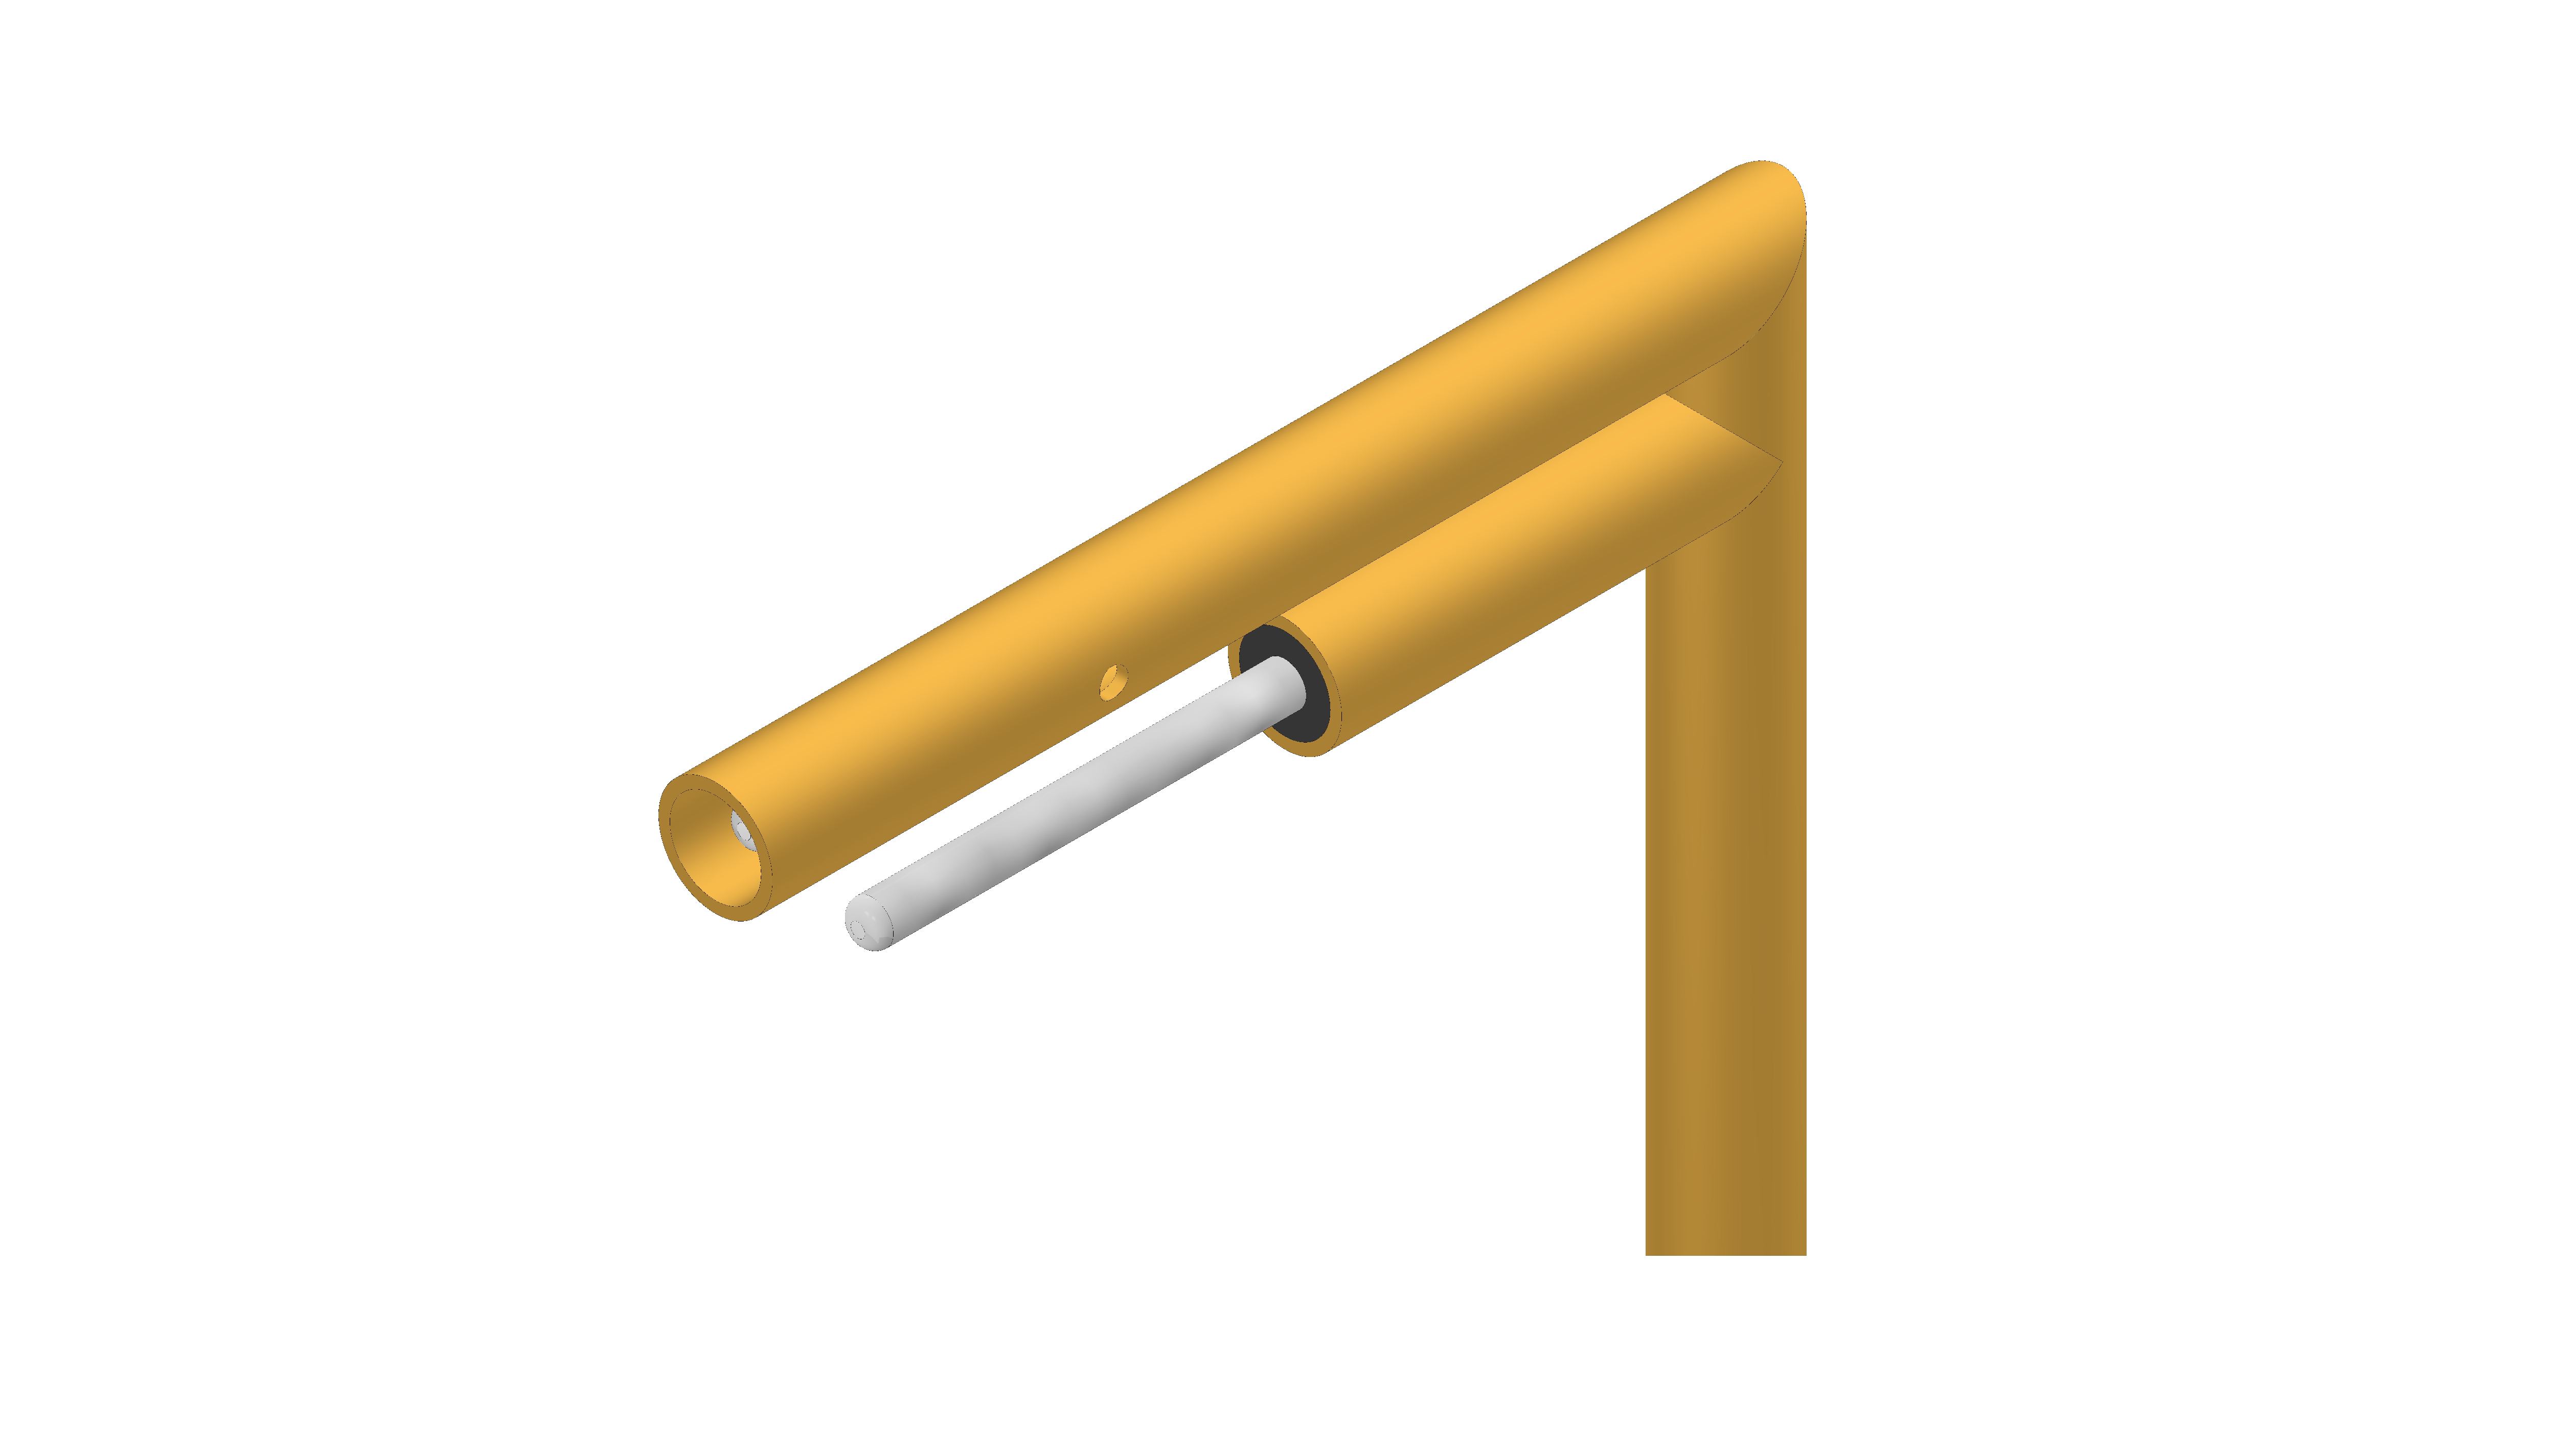
\includegraphics[width=\textwidth]{400_SIMULACE_KONSTRUKCNICH_UPRAV/Vykresy_rendery/Sonda_bez_stineni_B.png}
            \caption{Sonda bez stínění čidla B}
            \label{fig:sonda-bez-stineni-B}
        \end{figure}
        
        Zkoumáno bylo chování restitučních faktorů při různých rychlostech nabíhajícího proudu v rozmezí $100 \div 325 \unit{\frac{m}{s}}$ s krokem $25 \Unit{\frac{m}{s}}$ a při vychýlení sondy ve dvou rovinách – v rovině symetrie $XY$ (natočení značeno jako $\varphi _Z$) a poté kolmo na rovinu symetrie (rovina $XZ$, značeno $\varphi _Y$), v obou případech s krokem $2.5^o$ v rozmezí $\pm 15^o$.
                
        \subsubsection{Chování při různých rychlostech proudění}
            Výsledky výpočtu jsou znázorněny v obrázku \ref{fig:sonda-bez-stineni-rychlosti}. Z průběhu restitučního faktoru čidla B lze usuzovat, že docházelo k výraznějšímu ovlivnění proudění v jeho blízkosti vlivem stínění čidla A. To je patrné i z obrázku \ref{fig:sonda-bez-stineni-vizualizace}. 
            
            \begin{figure}[ht!]
                \centering
                \includegraphics*[width=\textwidth, trim={5.9cm 1.0cm 2.7cm 2.0cm}]{400_SIMULACE_KONSTRUKCNICH_UPRAV/Grafy/01_rychlosti.eps}
                \caption{Závislost restitučních faktorů sondy bez stínění čidla B na rychlosti proudění.}
                \label{fig:sonda-bez-stineni-rychlosti}
            \end{figure}

            \begin{figure}[ht!]
                \centering
                \begin{subfigure}{0.45\textwidth}
                    \centering
                    \captionsetup{width=.9\linewidth}
                    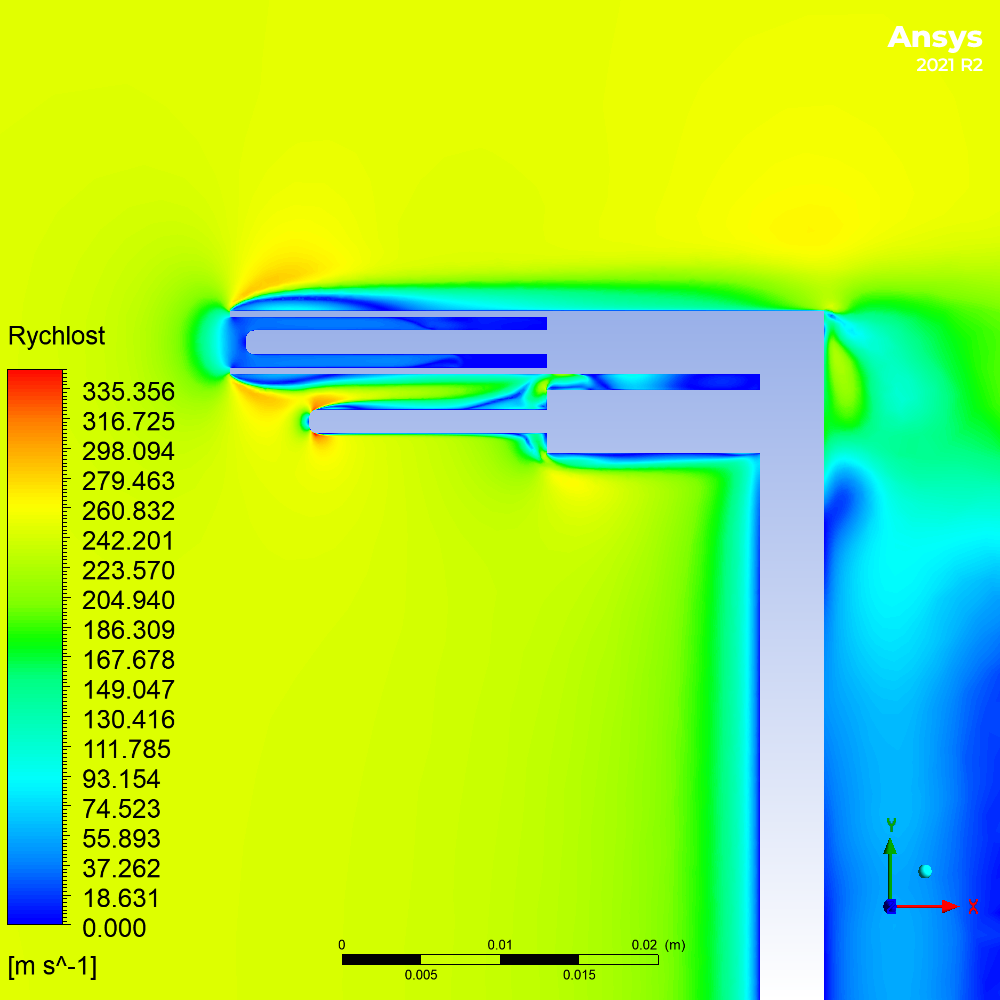
\includegraphics[width=\textwidth]{400_SIMULACE_KONSTRUKCNICH_UPRAV/Vizualizace/sonda_bez_stineni_vizualizace_rychlost.png}
                    \caption{Rychlostní pole.}
                \end{subfigure}
                \begin{subfigure}{0.45\textwidth}
                    \centering
                    \captionsetup{width=.9\linewidth}
                    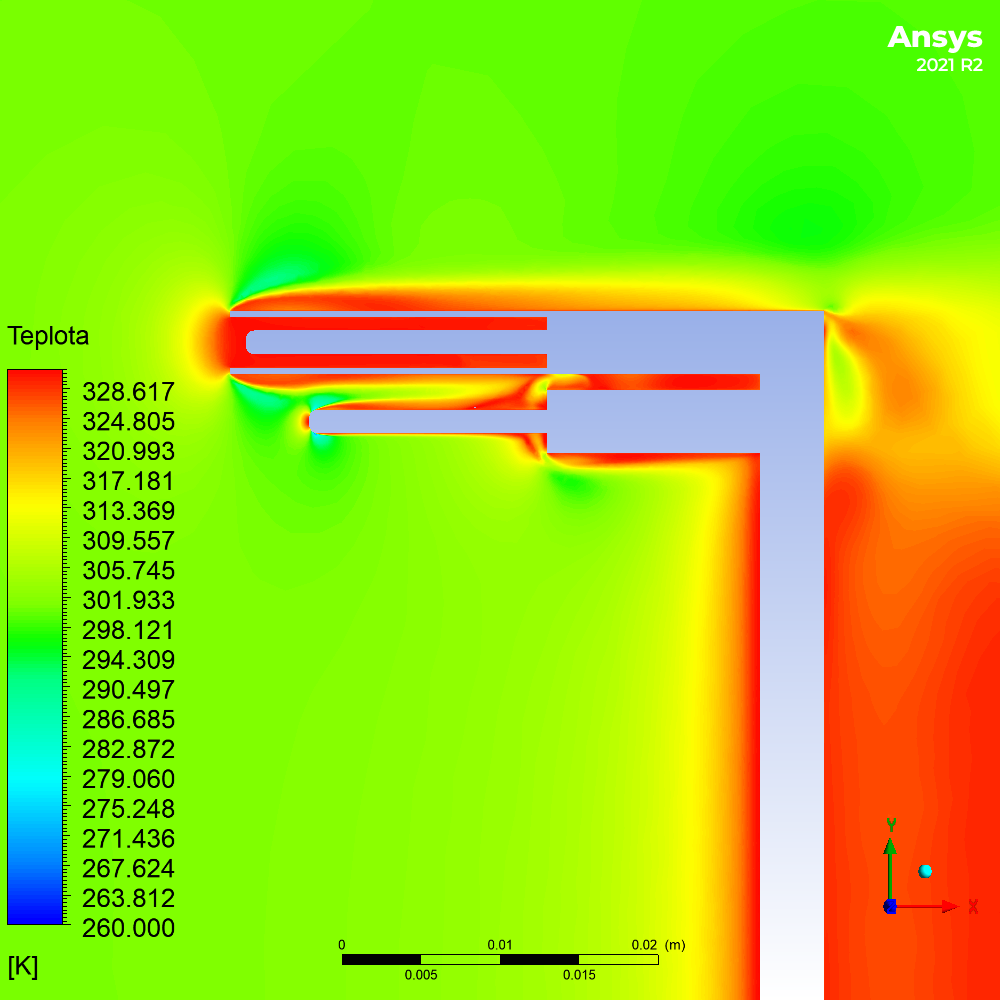
\includegraphics[width=\textwidth]{400_SIMULACE_KONSTRUKCNICH_UPRAV/Vizualizace/sonda_bez_stineni_vizualizace_teplota.png}
                    \caption{Teplotní pole.}
                \end{subfigure}
                \caption{Vizualizace vypočtených dat pro sondu bez stínění čidla B v rovině symetrie pro rychlost proudění $250 \Unit{\frac{m}{s}}$.}
                \label{fig:sonda-bez-stineni-vizualizace}
            \end{figure}


        \newpage
        \subsubsection{Směrová citlivost v rovině symetrie}
            Při natáčení sondy směrem dolů (tedy v záporném smyslu otáčení, kdy proud směřuje na vršek sondy) docházelo k zastínění čidla B, které se tak nacházelo částečně v úplavu trubice stínící čidlo A. To způsobilo výraznou změnu jeho restitučního faktoru, jak je patrné z obrázku \ref{fig:sonda-bez-stineni-rovina-symetrie} – relativní odchylka od hodnoty nevychýlené sondy byla pro natočení $-15^o$ rovna $7.4 \Unit{\%}$. Při natočení sondy opačným směrem nedocházelo k výrazným výchylkám restitučních faktorů, zde relativní odchylka nepřekročila $0.2 \Unit{\%}$.
            
            \begin{figure}[ht!]
                \centering
                \includegraphics*[width=\textwidth, trim={5.9cm 1.0cm 2.7cm 2.0cm}]{400_SIMULACE_KONSTRUKCNICH_UPRAV/Grafy/01_rovina_symetrie}
                \caption{Závislost restitučních faktorů sondy bez stínění čidla B na natočení sondy v rovině symetrie.}
                \label{fig:sonda-bez-stineni-rovina-symetrie}
            \end{figure}
        \subsubsection{Směrová citlivost kolmo na rovinu symetrie}
            Vychýlení sondy kolmo na rovinu symetrie neukázalo žádné vážné problémy (viz obrázek \ref{fig:sonda-bez-stineni-kolma-rovina}). Nejvyšší relativní odchylka restitučních faktorů nepřekročila $1.4 \Unit{\%}$ u čidla A a $1.8 \Unit{\%}$ u čidla B.
            
             \begin{figure}[ht!]
                \centering
                \includegraphics*[width=\textwidth, trim={5.9cm 1.0cm 2.7cm 2.0cm}]{400_SIMULACE_KONSTRUKCNICH_UPRAV/Grafy/01_kolma_rovina}
                \caption{Závislost restitučních faktorů sondy bez stínění čidla B na natočení kolmo na rovinu symetrie.}
                \label{fig:sonda-bez-stineni-kolma-rovina}
            \end{figure}

        \subsubsection{Zhodnocení}
            Problematickým místem první verze sondy se ukázalo čidlo B, které bylo ovlivňováno stíněním čidla A jak při změnách rychlosti proudění, tak při změnách natočení sondy. Prvním návrhem konstrukční úpravy tak bylo jeho odstínění.
    
    \subsection{Sonda se stíněním čidla B}
        Odstínění čidla B bylo zajištěno pomocí trubice $5.8 \times 0.4 \Unit{mm}$ uchycené ke stínění čidla A, viz obrázek \ref{fig:sonda-se-stinenim-B}. Detailní geometrie spolu s použitými rozměry modelu jsou uvedeny v příloze \ref{fig:sonda-se-stinenim-B-vykres}. 
        
        \begin{figure}[ht!]
            \centering
            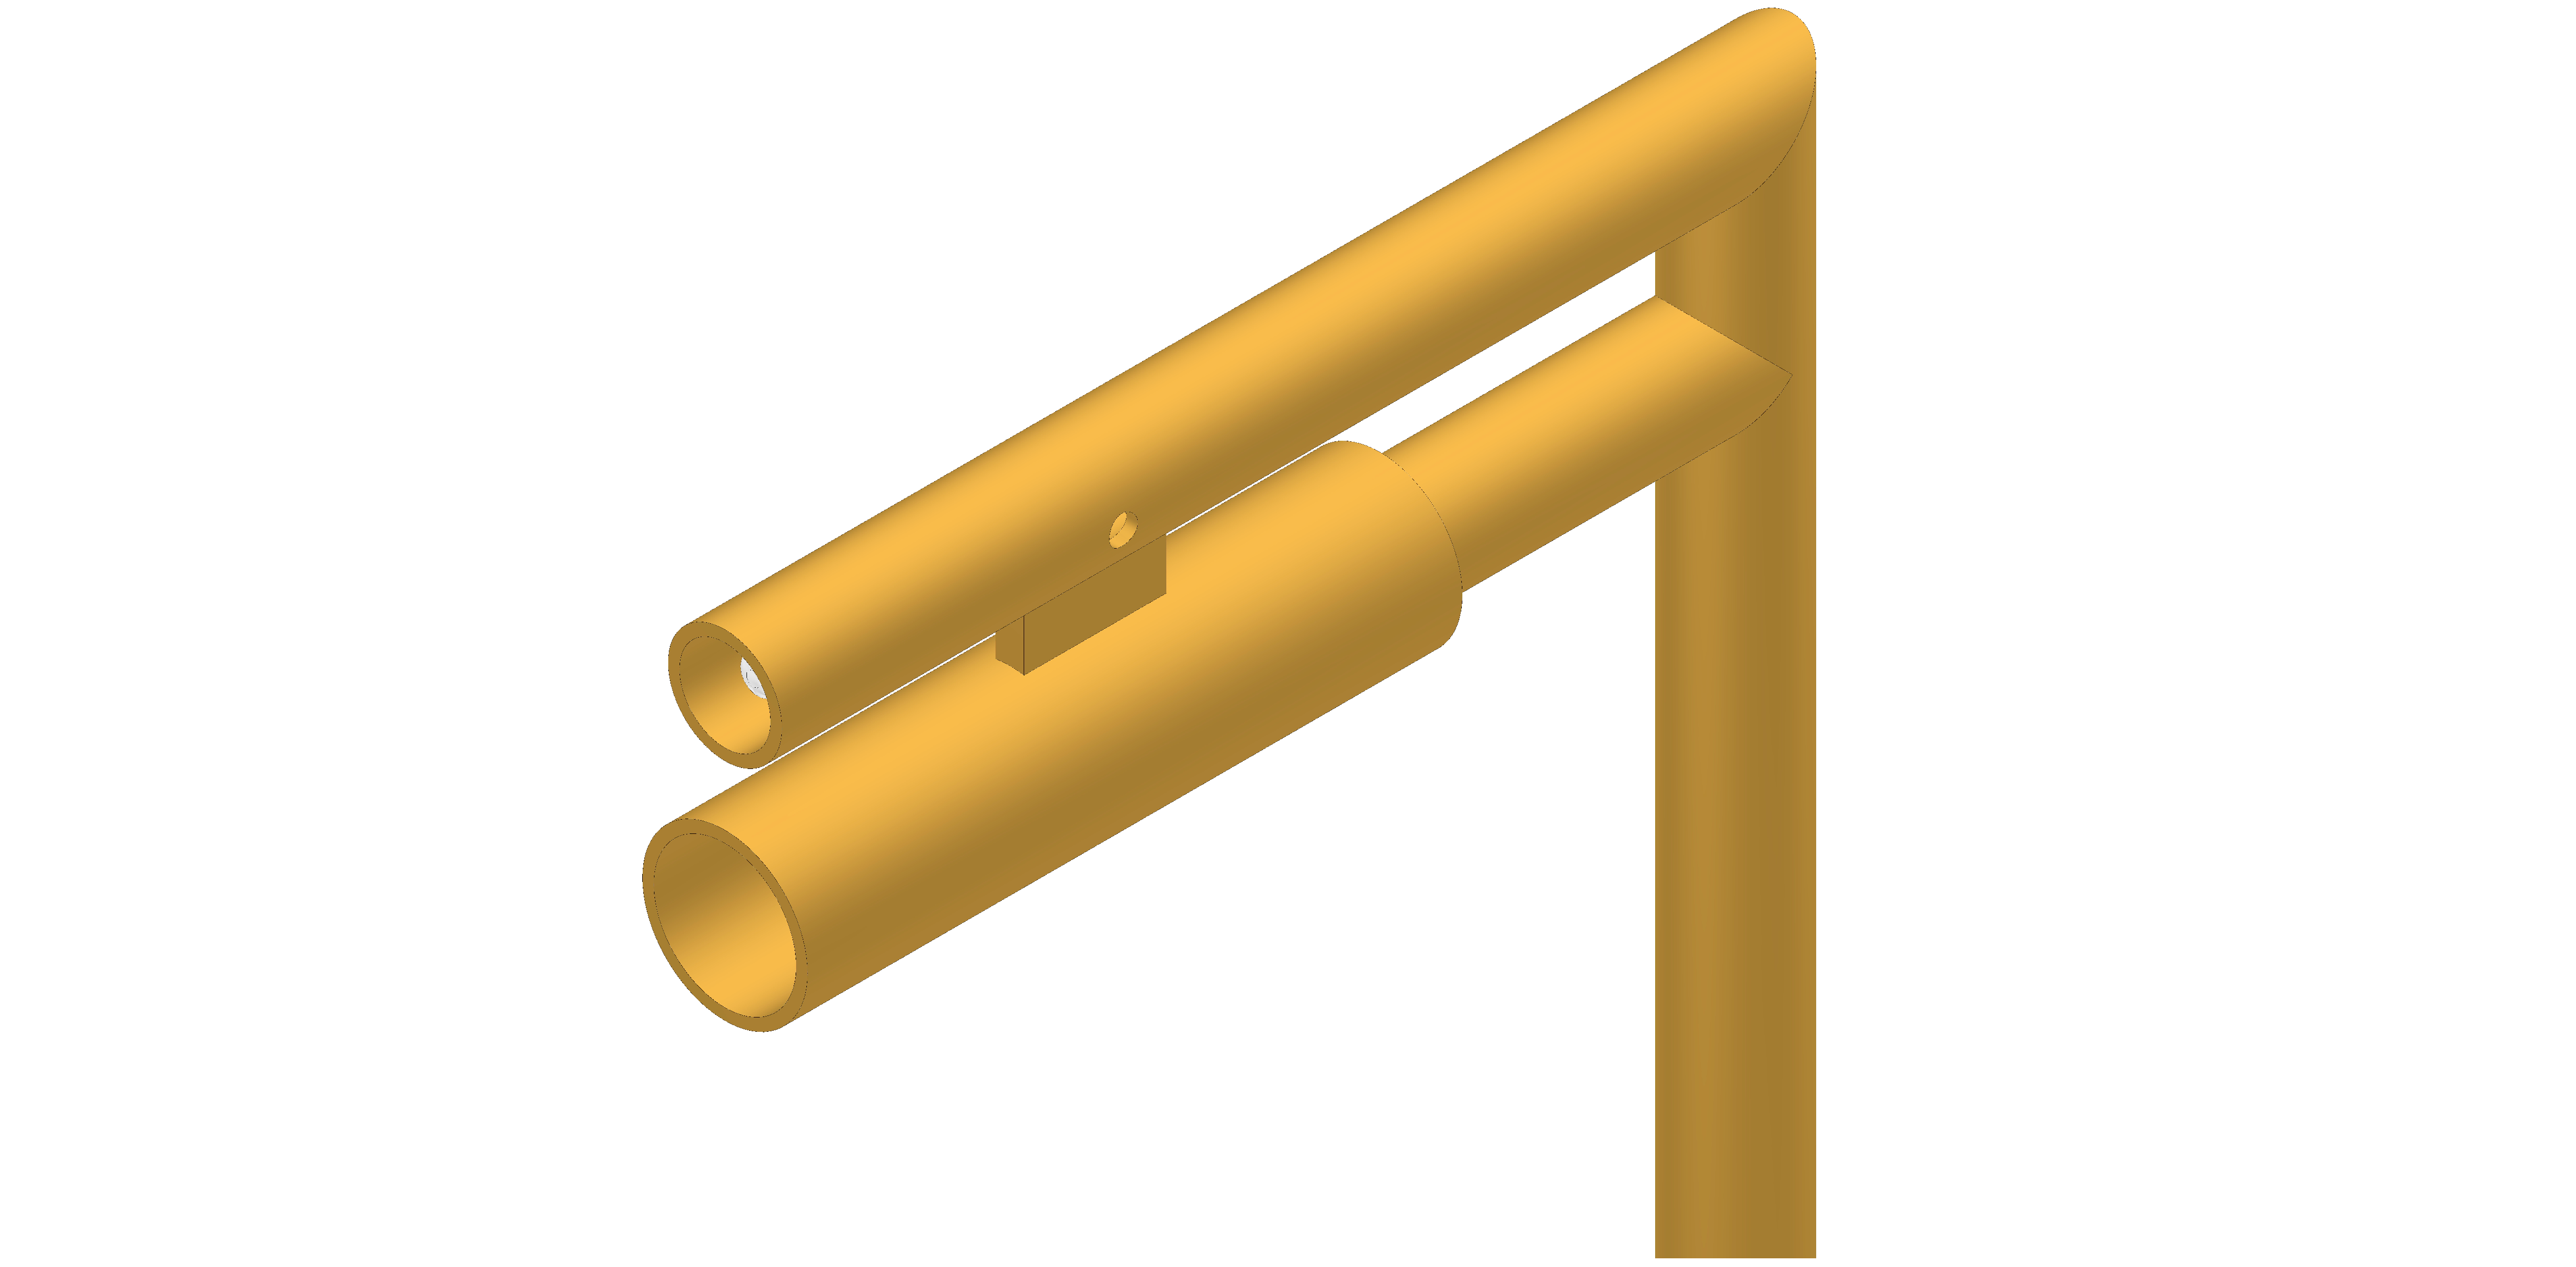
\includegraphics[width=\textwidth]{400_SIMULACE_KONSTRUKCNICH_UPRAV/Vykresy_rendery/Sonda_se_stinenim_B.png}
            \caption{Sonda se stíněním čidla B}
            \label{fig:sonda-se-stinenim-B}
        \end{figure}

        Pro tuto geometrii byl proveden pouze jeden výpočet, a to pro rychlost $250 \Unit{\frac{m}{s}}$. Důvodem byla volba příliš úzké stínící trubice, která způsobovala výrazně vyšší ohřev čidla B oproti původní verzi (restituční faktor narostl o $7.3 \Unit{\%})$. 

        \begin{figure}[ht!]
            \centering
            \begin{subfigure}{0.45\textwidth}
                \centering
                \captionsetup{width=.9\linewidth}
                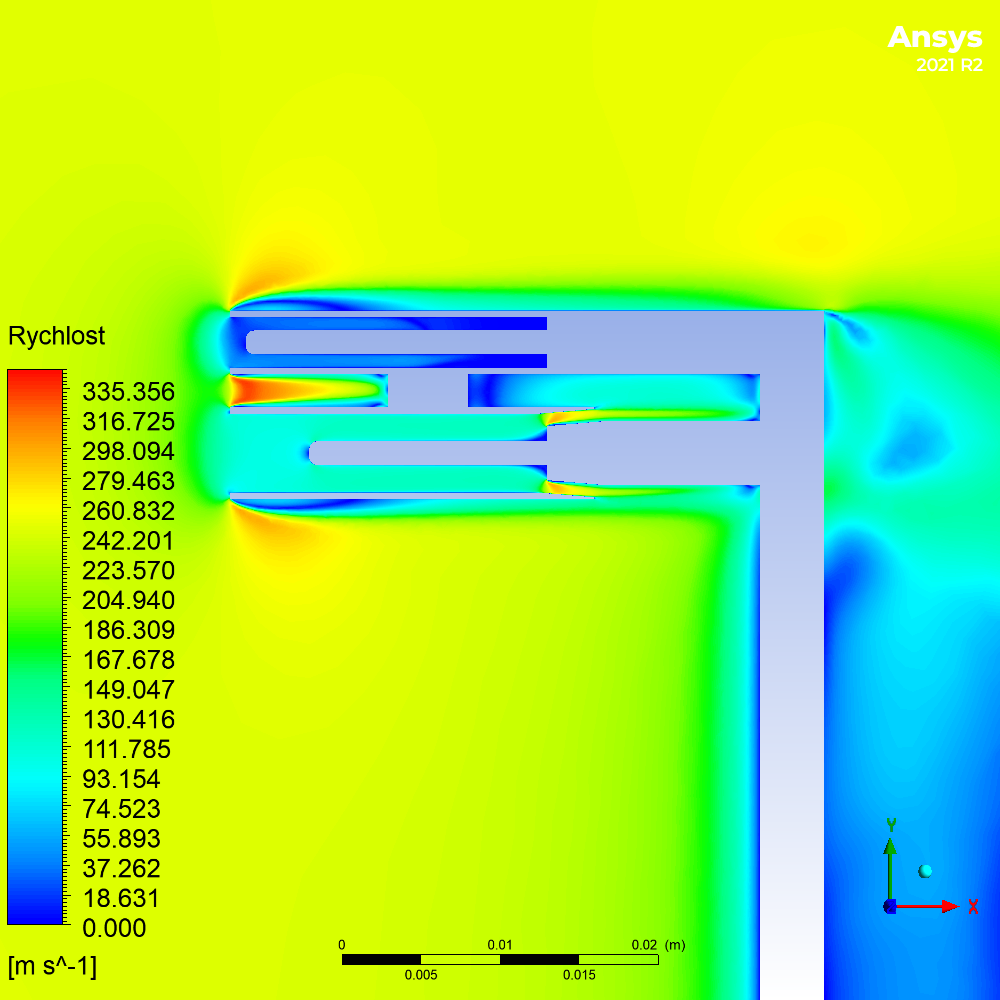
\includegraphics[width=\textwidth]{400_SIMULACE_KONSTRUKCNICH_UPRAV/Vizualizace/sonda_se_stinenim_B_vizualizace_rychlost.png}
                \caption{Rychlostní pole.}
            \end{subfigure}
            \begin{subfigure}{0.45\textwidth}
                \centering
                \captionsetup{width=.9\linewidth}
                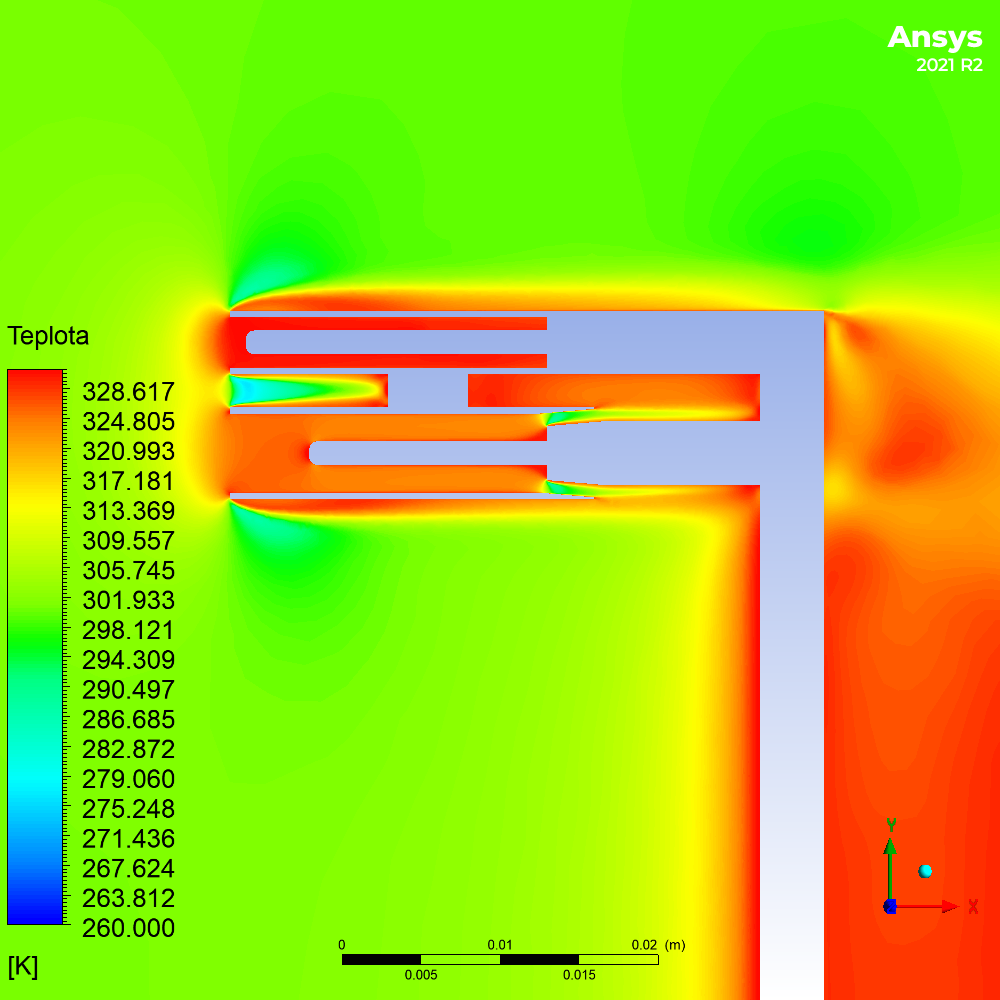
\includegraphics[width=\textwidth]{400_SIMULACE_KONSTRUKCNICH_UPRAV/Vizualizace/sonda_se_stinenim_B_vizualizace_teplota.png}
                \caption{Teplotní pole.}
            \end{subfigure}
            \caption{Vizualizace vypočtených dat pro sondu se stíněním čidla B v rovině symetrie pro rychlost proudění $250 \Unit{\frac{m}{s}}$.}
            \label{fig:sonda-se-stinenim-B-vizualizace}
        \end{figure}
    
    \newpage
    \subsection{Sonda s rozšířeným stíněním čidla B}
        Oproti předchozí úpravě došlo pouze ke zvětšení trubice stínící čidlo B – místo původního rozměru byla použito stínění o vnějším průměru $8 \Unit{mm}$ a tloušťce stěny $0.45 \Unit{mm}$ (geometrie podrobně popsána v příloze \ref{fig:sonda-s-rozsirenym-stinenim-B-vykres}). Zde byl již ohřev čidla B přijatelný a bylo tak analyzováno chování sondy obdobně, jako v kapitole \ref{sec:sonda-bez-stineni-B} – byla zkoumána závislost restitučních faktorů na rychlosti proudění v rozmezí $125 \div 325 \Unit{\frac{m}{s}}$ a na natočení v rovině symetrie a kolmo na ní, opět v rozsahu $\pm 15^o$.
        
        \begin{figure}[ht!]
            \centering
            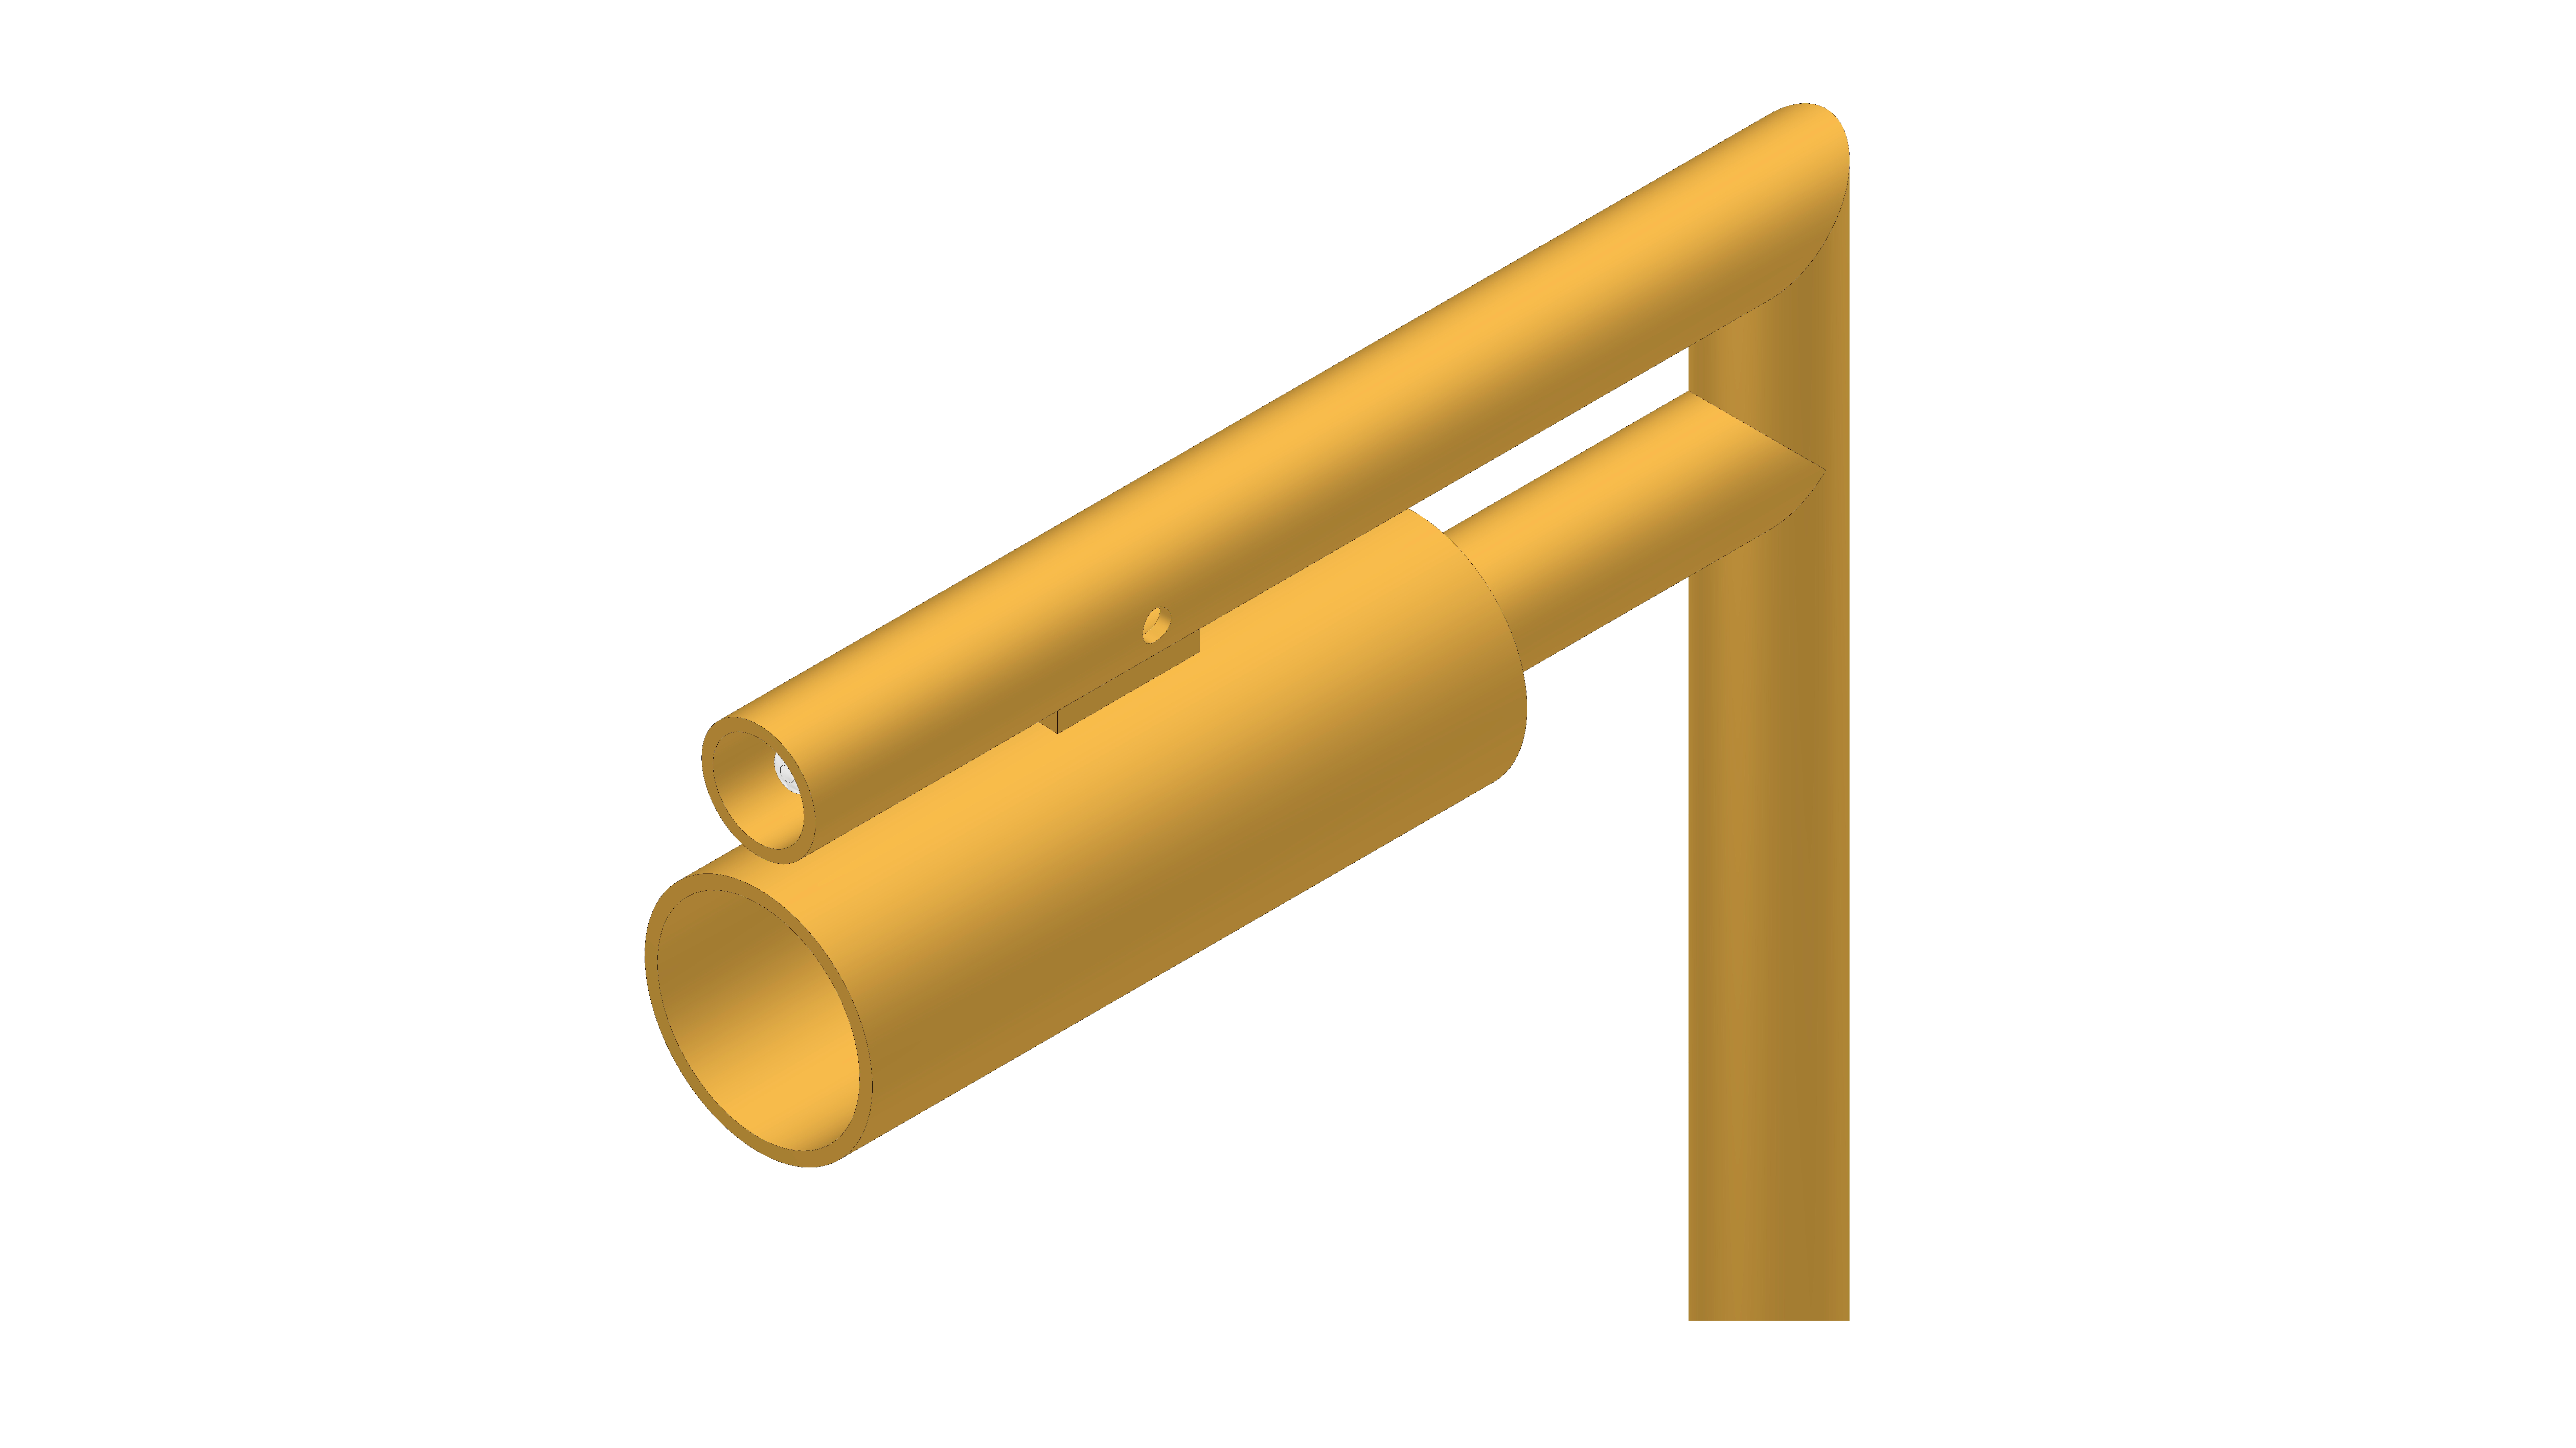
\includegraphics[width=\textwidth]{400_SIMULACE_KONSTRUKCNICH_UPRAV/Vykresy_rendery/Sonda_s_rozsirenym_stinenim_B.png}
            \caption{Sonda se stíněním čidla B}
            \label{fig:sonda-s-rozsirenym-stinenim-B}
        \end{figure}
        
        \subsubsection{Chování při různých rychlostech proudění}
            Výsledky výpočtu shrnuje obrázek \ref{fig:sonda-s-rosirenym-stinenim-rychlosti}. Přidáním stínící trubice došlo ke snížení vlivu stínění čidla A, nicméně za cenu zvýšení restitučního faktoru čidla B, a to o přibližně $5 \Unit{\%}$.
            
            \begin{figure}[ht!]
                \centering
                \includegraphics*[width=\textwidth, trim={5.9cm 1.0cm 2.7cm 2.0cm}]{400_SIMULACE_KONSTRUKCNICH_UPRAV/Grafy/03_rychlosti.eps}
                \caption{Závislost restitučních faktorů sondy s rozšířeným stíněním čidla B na rychlosti proudění}
                \label{fig:sonda-s-rosirenym-stinenim-rychlosti}
            \end{figure}

            \begin{figure}[ht!]
                \centering
                \begin{subfigure}{0.45\textwidth}
                    \centering
                    \captionsetup{width=.9\linewidth}
                    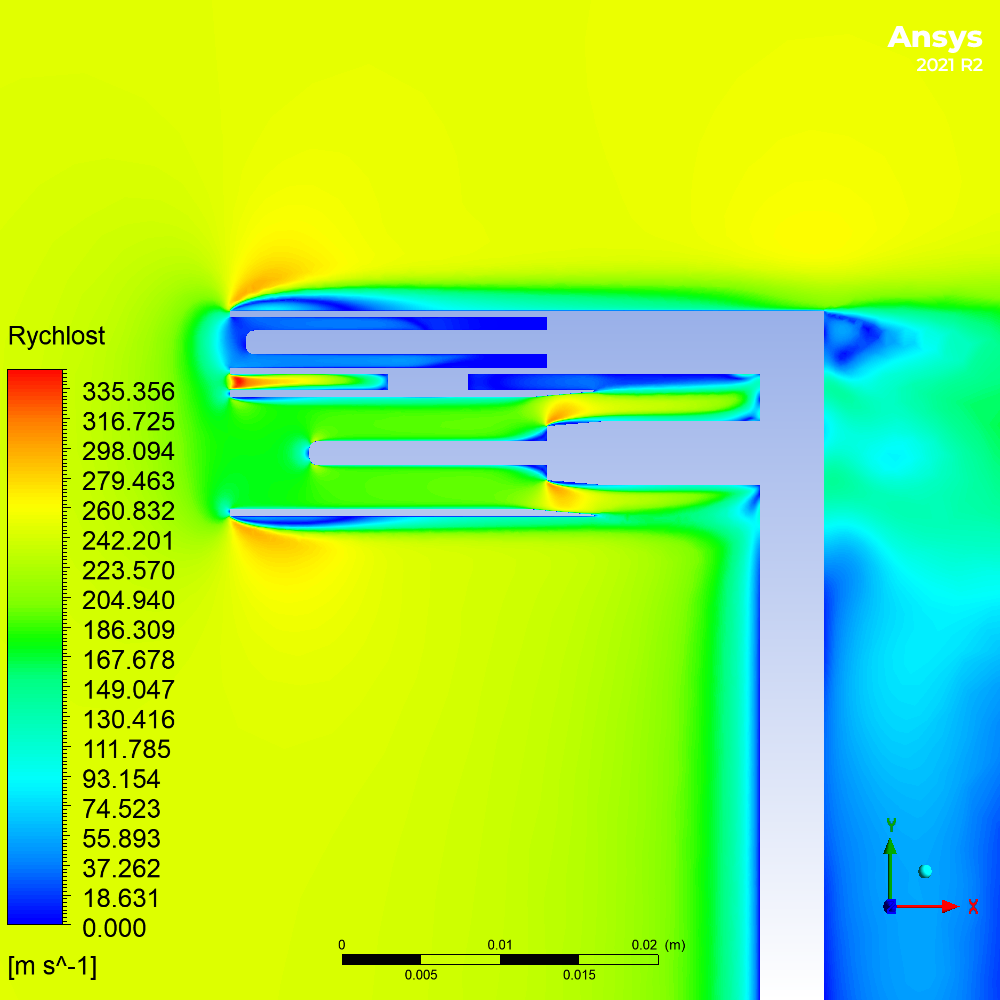
\includegraphics[width=\textwidth]{400_SIMULACE_KONSTRUKCNICH_UPRAV/Vizualizace/sonda_s_rozsirenym_stinenim_B_vizualizace_rychlost.png}
                    \caption{Rychlostní pole.}
                \end{subfigure}
                \begin{subfigure}{0.45\textwidth}
                    \centering
                    \captionsetup{width=.9\linewidth}
                    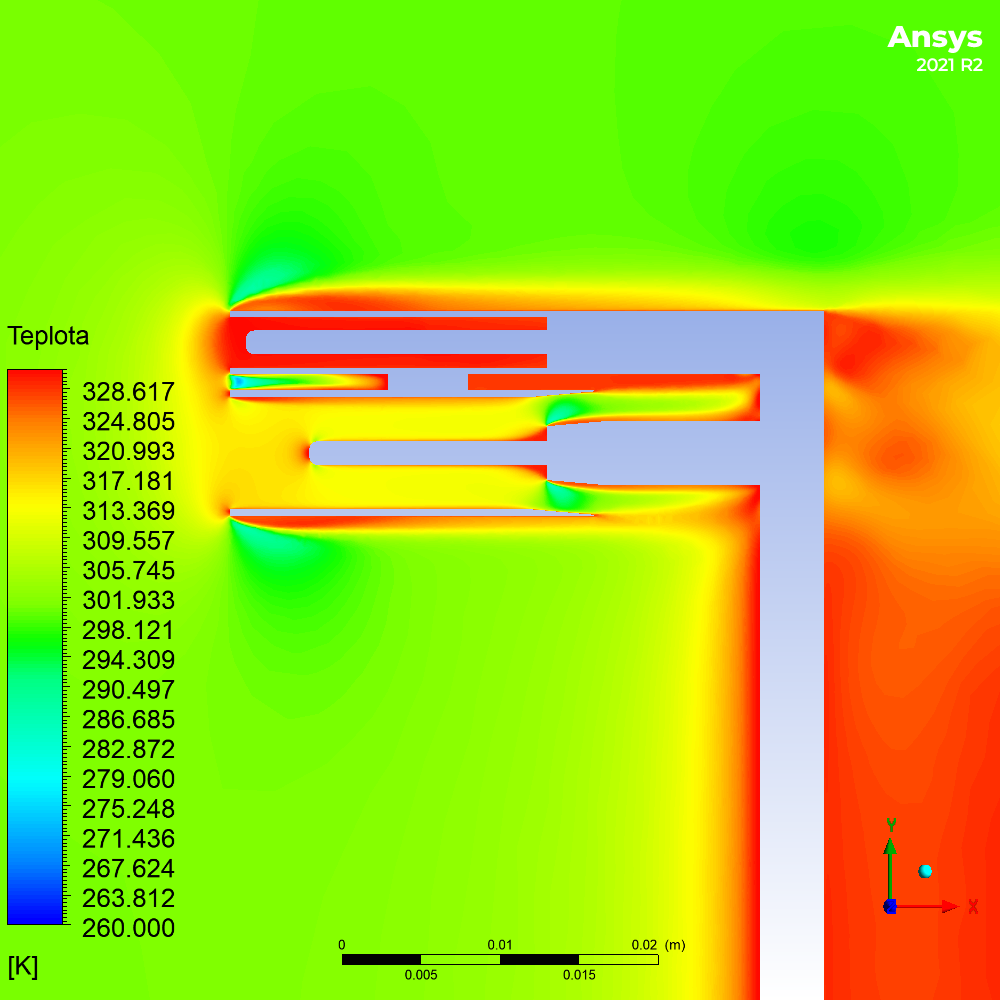
\includegraphics[width=\textwidth]{400_SIMULACE_KONSTRUKCNICH_UPRAV/Vizualizace/sonda_s_rozsirenym_stinenim_B_vizualizace_teplota.png}
                    \caption{Teplotní pole.}
                \end{subfigure}
                \caption{Vizualizace vypočtených dat pro sondu s rozšířeným stíněním čidla B v rovině symetrie pro rychlost proudění $250 \Unit{\frac{m}{s}}$.}
                \label{fig:sonda-s-rozsirenym-stinenim-B-vizualizace}
            \end{figure}
        \subsubsection{Směrová citlivost v rovině symetrie}
            Zde bylo zlepšení vlivem přidání stínění nejpatrnější. Restituční faktor čidla B se oproti variantě sondy bez stínění (kapitola \ref{sec:sonda-bez-stineni-B}) při natáčení v rovině symetrie prakticky neměnil, viz obrázek \ref{fig:sonda-s-rosirenym-stinenim-rovina-symetrie}.
            
            \begin{figure}[ht!]
                \centering
                \includegraphics*[width=\textwidth, trim={5.9cm 1.0cm 2.7cm 2.0cm}]{400_SIMULACE_KONSTRUKCNICH_UPRAV/Grafy/03_rovina_symetrie}
                \caption{Závislost restitučních faktorů sondy s rozšířeným stíněním čidla B na natočení sondy v rovině symetrie}
                \label{fig:sonda-s-rosirenym-stinenim-rovina-symetrie}
            \end{figure}
        \subsubsection{Směrová citlivost kolmo na rovinu symetrie}
            Výsledky výpočtů, reprezentovány na obrázku \ref{fig:sonda-s-rosirenym-stinenim-kolma-rovina}, představovaly i v tomto případě zlepšení chování restitučního faktoru čidla B, nebylo však tak výrazné, jako při natáčení sondy v rovině symetrie.
            
             \begin{figure}[ht!]
                \centering
                \includegraphics*[width=\textwidth, trim={5.9cm 1.0cm 2.7cm 2.0cm}]{400_SIMULACE_KONSTRUKCNICH_UPRAV/Grafy/03_kolma_rovina}
                \caption{Závislost restitučních faktorů sondy s rozšířeným stíněním čidla B na natočení kolmo na rovinu symetrie}
                \label{fig:sonda-s-rosirenym-stinenim-kolma-rovina}
            \end{figure}

        \subsubsection{Zhodnocení}
            Přidáním stínění k čidlu B došlo ke snížení směrové citlivosti sondy a k zmenšení vlivu stínění čidla A na restituční faktor čidla B. Negativním dopadem této úpravy geometrie byl vyšší ohřev čidla B, dalším krokem analýzy konstrukčních úprav tak bylo detailnější zkoumání vlivu průměru stínění čidla B na jeho restituční faktor.
        
    \newpage
    \subsection{Vliv průměru stínění čidla B}
        DATA
        
        \begin{figure}[ht!]
            \centering
            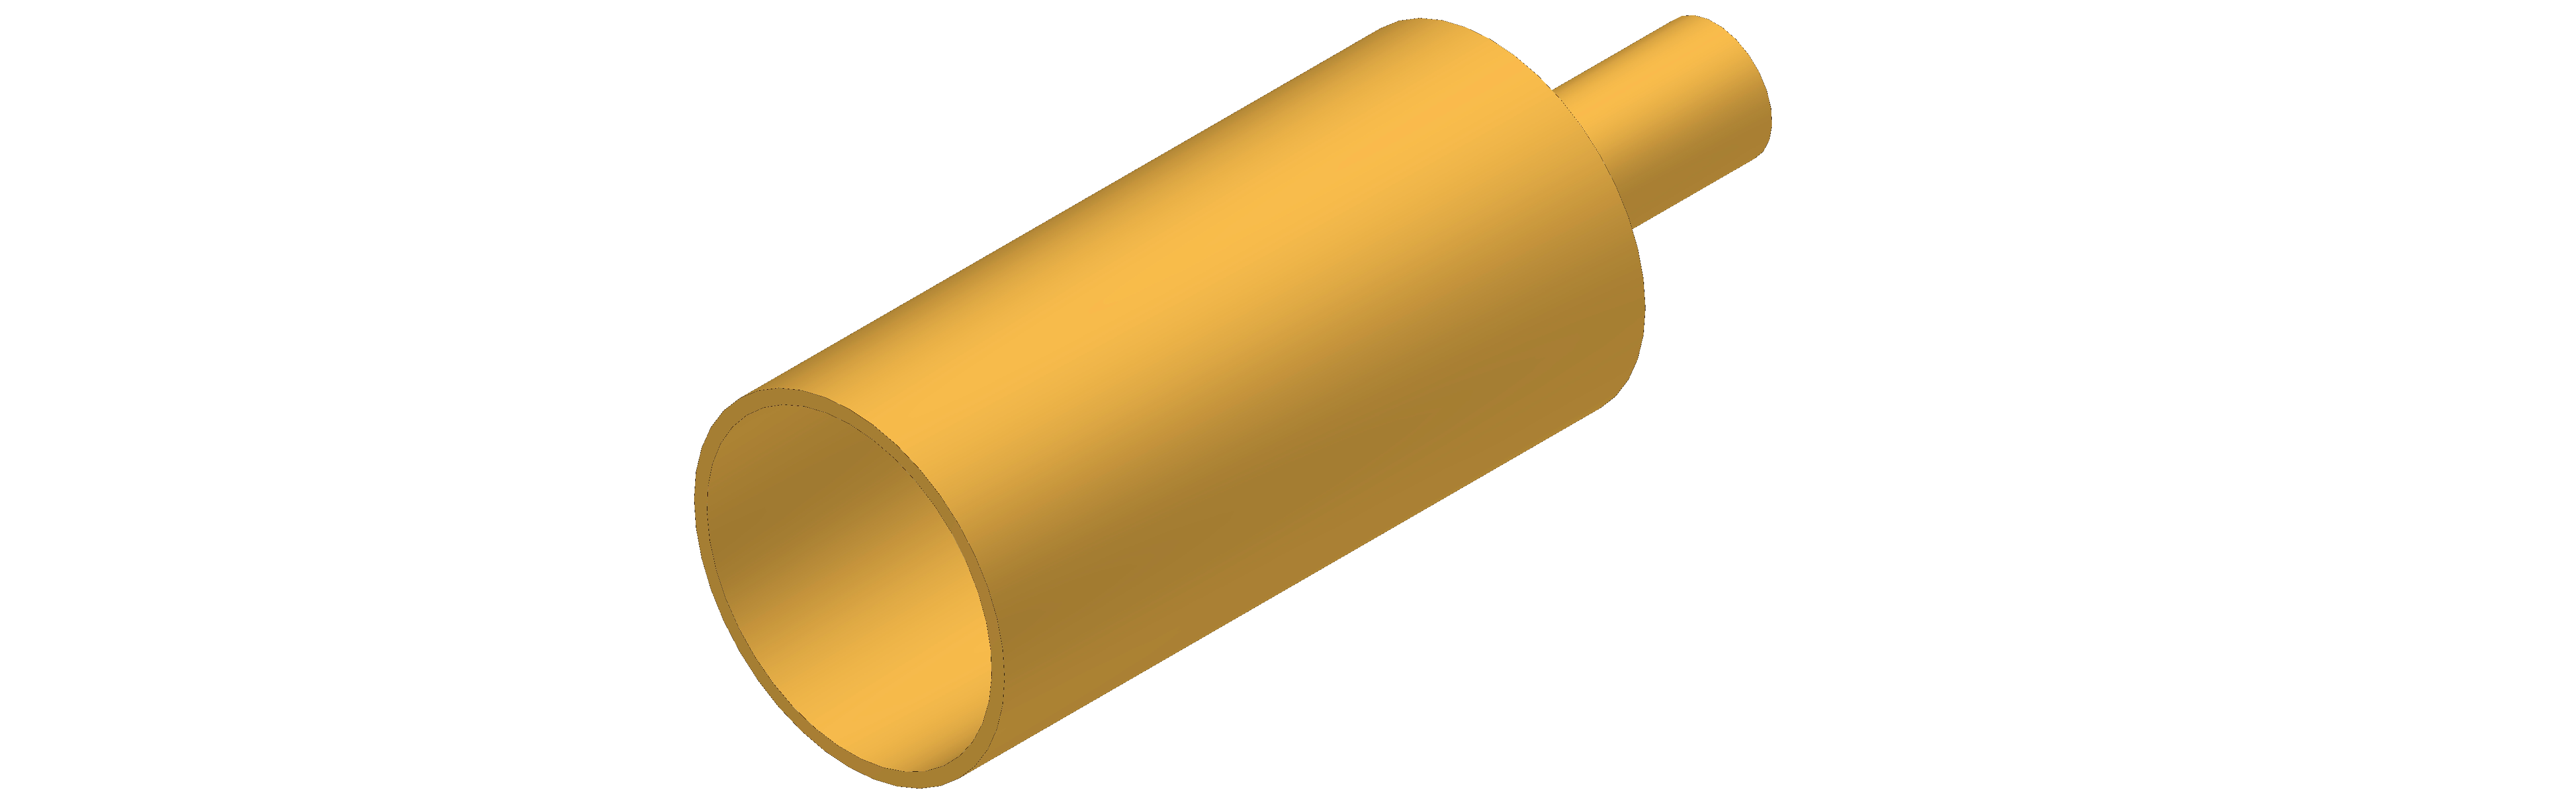
\includegraphics[width=\textwidth]{400_SIMULACE_KONSTRUKCNICH_UPRAV/Vykresy_rendery/Stineni_B.png}
            \caption{Stínění čidla B}
            \label{fig:stineni-B}
        \end{figure}
        
        
        \begin{figure}[ht!]
            \centering
            \includegraphics*[width=\textwidth, trim={5.9cm 1.0cm 5.8cm 2.0cm}]{400_SIMULACE_KONSTRUKCNICH_UPRAV/Grafy/04_prumer_stineni_B}
            \caption{Závislost restitučního faktoru čidla B na průměru stínění}
            \label{fig:prumer-stineni-B}
        \end{figure}
    
    \newpage
    \subsection{Vliv průměru stínění čidla A} \label{sec:stineni-A}
        DATA
        
        \begin{figure}[ht!]
            \centering
            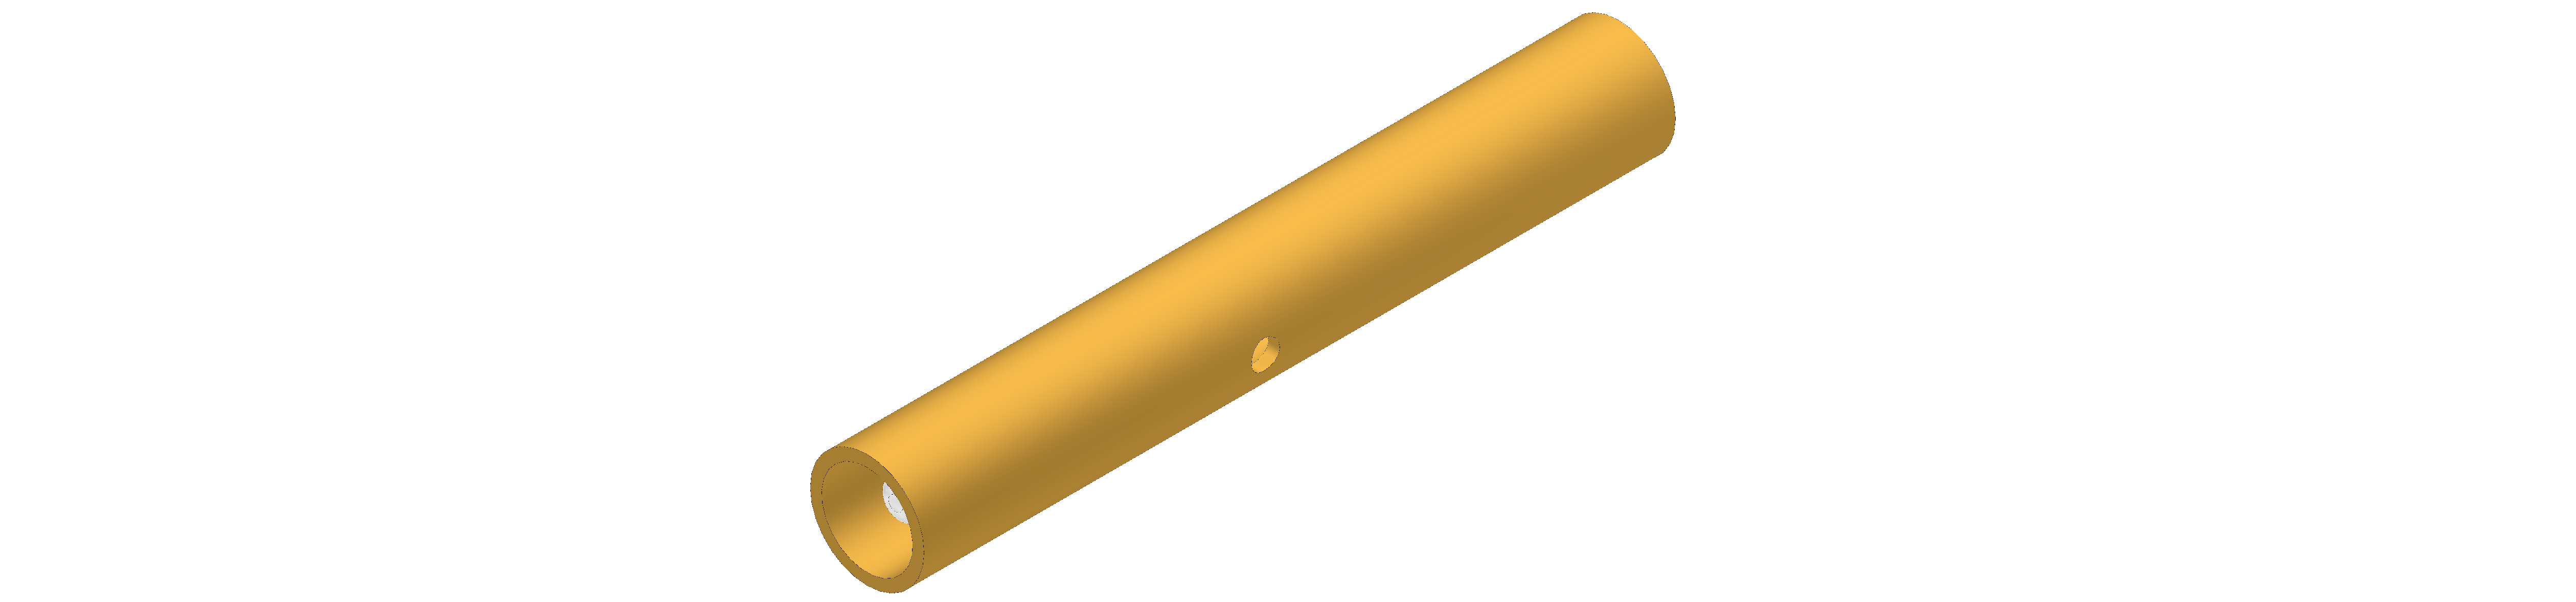
\includegraphics[width=\textwidth]{400_SIMULACE_KONSTRUKCNICH_UPRAV/Vykresy_rendery/Stineni_A.png}
            \caption{Stínění čidla A}
            \label{fig:stineni-A}
        \end{figure}
        
        \begin{figure}[ht!]
            \centering
            \includegraphics*[width=\textwidth, trim={5.25cm 1.0cm 5.8cm 2.0cm}]{400_SIMULACE_KONSTRUKCNICH_UPRAV/Grafy/05_prumer_stineni_A}
            \caption{Závislost restitučního faktoru čidla A na průměru stínění}
            \label{fig:prumer-stineni-A}
        \end{figure}
    
   \newpage
     \subsection{Vliv polohy odvětrání čidla A}
        DATA
        
          \begin{figure}[ht!]
            \centering
            \includegraphics*[width=\textwidth, trim={5.25cm 1.0cm 5.8cm 2.0cm}]{400_SIMULACE_KONSTRUKCNICH_UPRAV/Grafy/06_poloha_odvetrani_A.eps}
            \caption{Závislost restitučního faktoru čidla A na poloze odvětrání}
            \label{fig:poloha-odvetrani-A}
        \end{figure}
    
    \newpage
    \subsection{Vliv průměru odvětrání čidla A}
        DATA
        
        \begin{figure}[ht!]
            \centering
            \includegraphics*[width=\textwidth, trim={5.25cm 1.0cm 5.8cm 2.0cm}]{400_SIMULACE_KONSTRUKCNICH_UPRAV/Grafy/07_prumer_odvetrani_A.eps}
            \caption{Závislost restitučního faktoru čidla A na průměru odvětrání}
            \label{fig:prumer-odvetrani-A}
        \end{figure}
    
    \newpage
    \subsection{Vliv přidání divergentního vstupu pro čidlo A}
        DATA
        
        \begin{figure}[ht!]
            \centering
            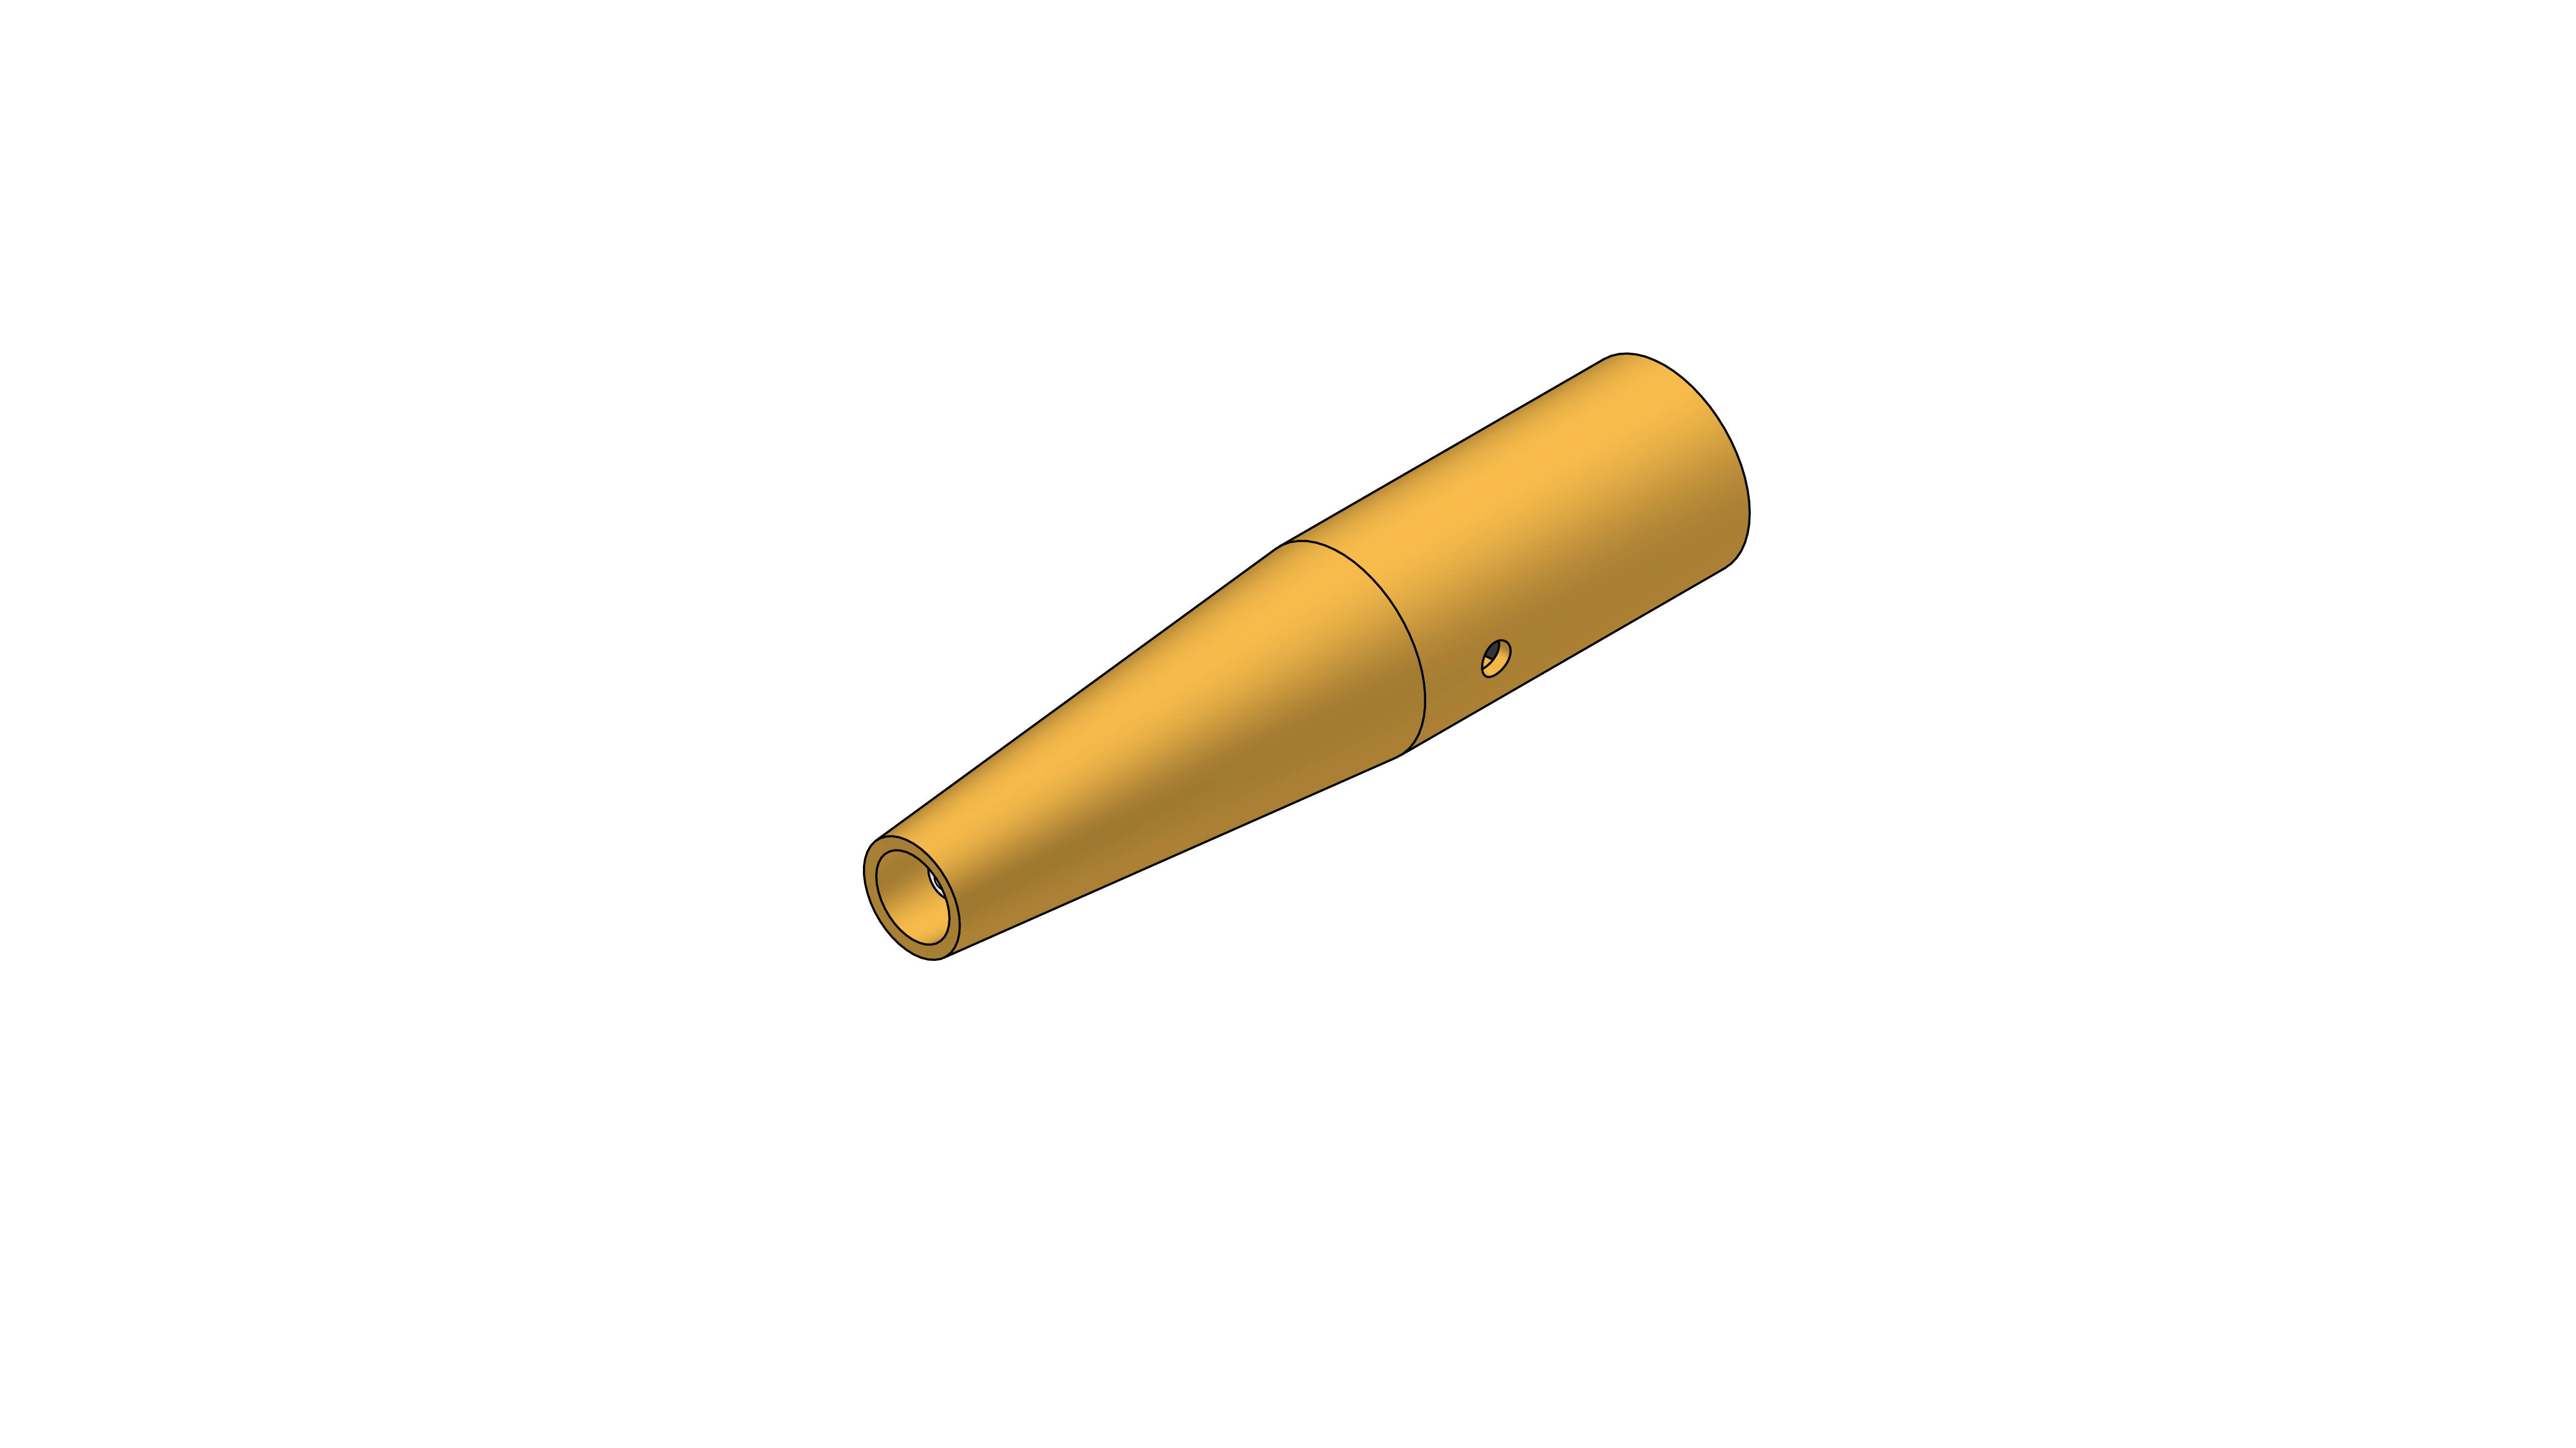
\includegraphics[width=\textwidth]{400_SIMULACE_KONSTRUKCNICH_UPRAV/Vykresy_rendery/Difuzor_A.png}
            \caption{Čidlo A s divergentním vstupem}
            \label{fig:difuzor-A}
        \end{figure}
    
        \begin{figure}[ht!]
            \centering
            \includegraphics*[width=\textwidth, trim={5.25cm 1.0cm 5.8cm 2.0cm}]{400_SIMULACE_KONSTRUKCNICH_UPRAV/Grafy/08_divergentni_cast_A.eps}
            \caption{Závislost restitučního faktoru čidla A na vrcholovém úhlu divergentního vstupu}
            \label{fig:divergentni-cast-A}
        \end{figure}
    
    \newpage
    \subsection{Vliv přidání kavity do stínění čidla A}
        DATA
        
        \begin{figure}[ht!]
            \centering
            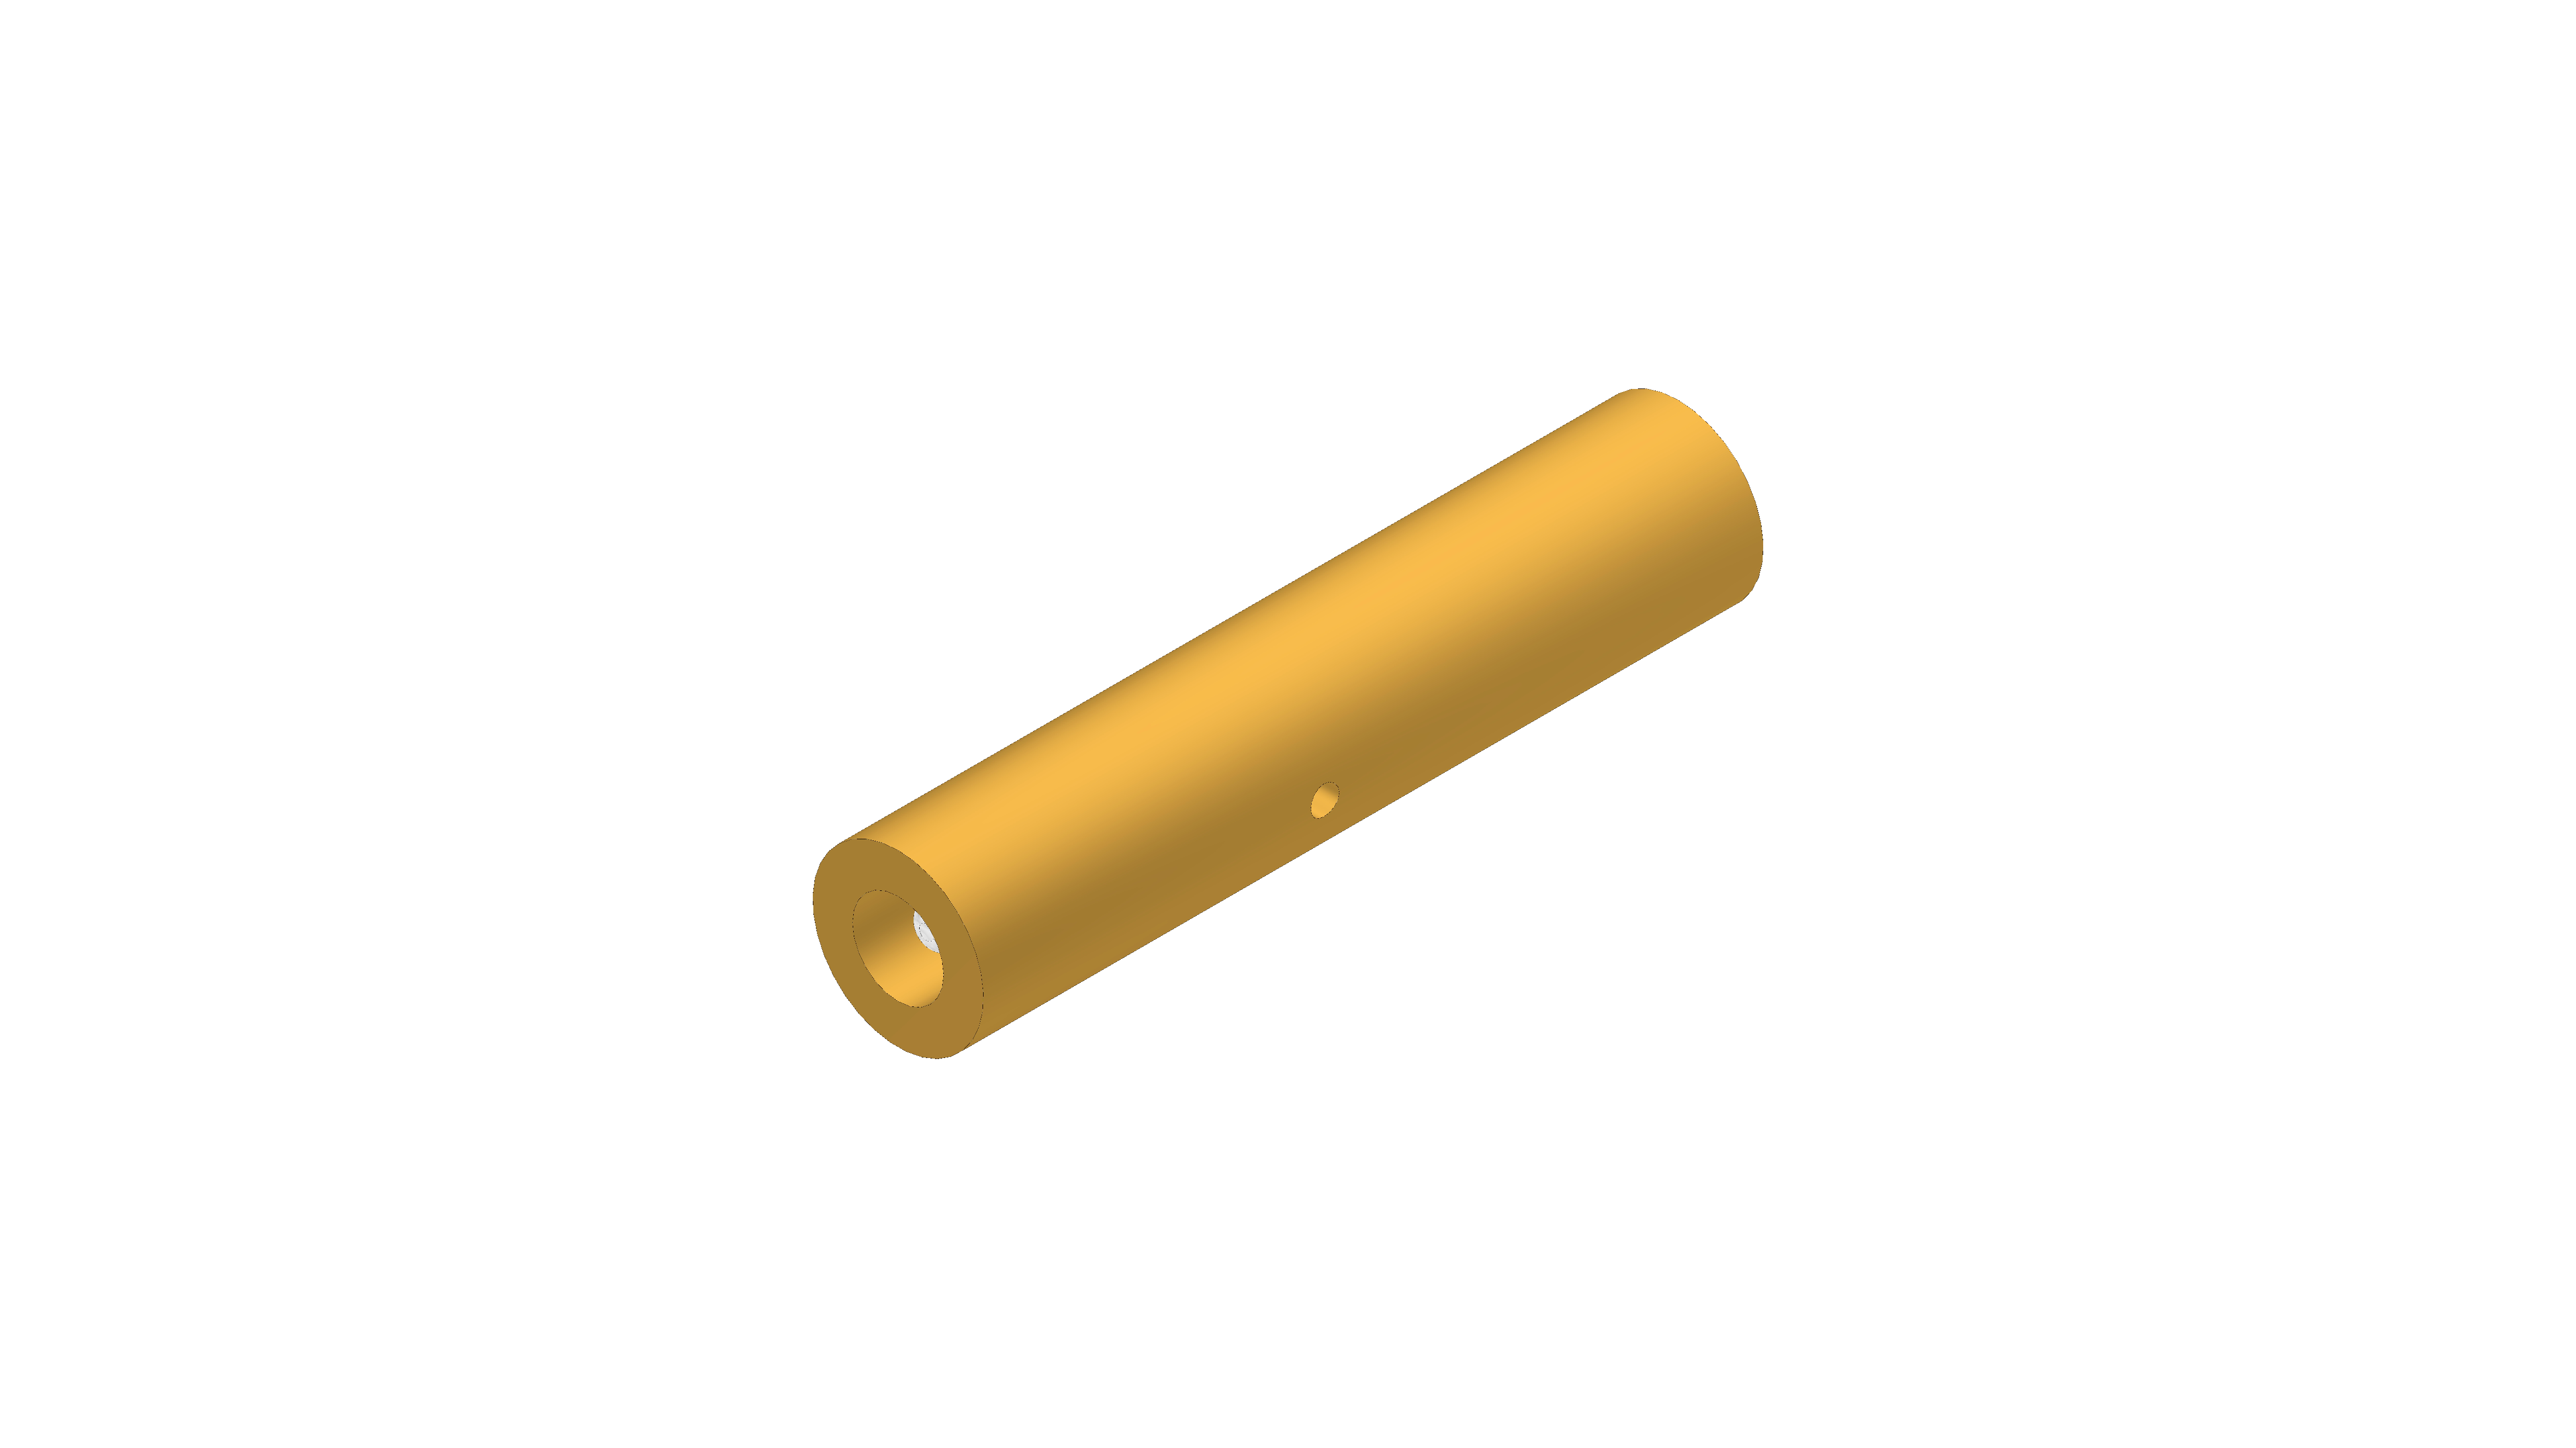
\includegraphics[width=\textwidth]{400_SIMULACE_KONSTRUKCNICH_UPRAV/Vykresy_rendery/Kavita.png}
            \caption{Čidlo A s přidanou kavitou do stínění}
            \label{fig:kavita-A}
        \end{figure}
    
        \begin{figure}[ht!]
            \centering
            \includegraphics*[width=\textwidth, trim={5.25cm 1.0cm 5.8cm 2.0cm}]{400_SIMULACE_KONSTRUKCNICH_UPRAV/Grafy/kavita.eps}
            \caption{Závislost restitučního faktoru čidla A na tloušťce kavity uvnitř stínění}
            \label{fig:kavita-A-graf}
        \end{figure}
    
    \newpage
    
    \subsection{Vliv přidání kavity do stínění čidla B}
        DATA
        
        \begin{figure}[ht!]
            \centering
            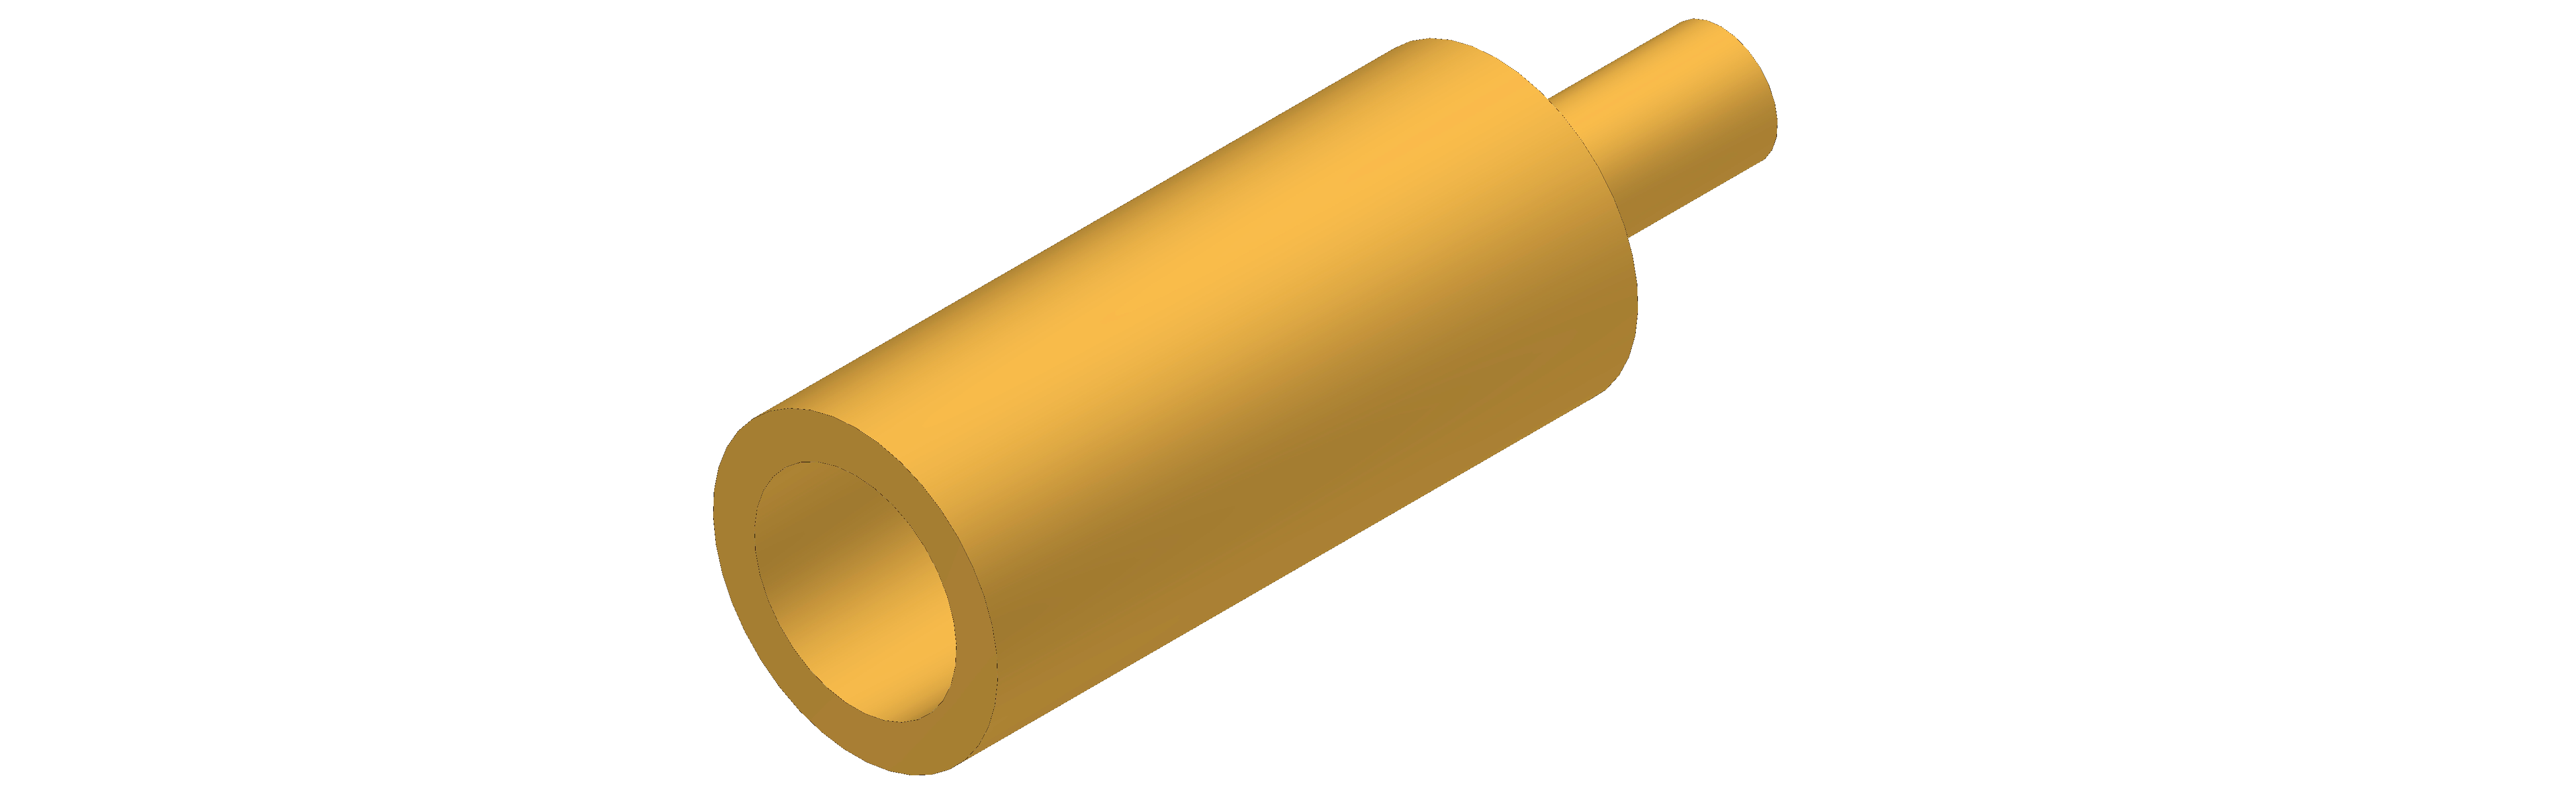
\includegraphics[width=\textwidth]{400_SIMULACE_KONSTRUKCNICH_UPRAV/Vykresy_rendery/Kavita_B.png}
            \caption{Čidlo B s přidanou kavitou do stínění}
            \label{fig:kavita-B}
        \end{figure}
    
        \begin{figure}[ht!]
            \centering
            \includegraphics*[width=\textwidth, trim={5.25cm 1.0cm 5.8cm 2.0cm}]{400_SIMULACE_KONSTRUKCNICH_UPRAV/Grafy/kavita_B.eps}
            \caption{Závislost restitučního faktoru čidla B na tloušťce kavity uvnitř stínění}
            \label{fig:kavita-B-graf}
        \end{figure}
    
    \newpage
    \subsection{Vliv materiálu trubice sondy}
        TODO
    